\documentclass{report}
\usepackage[lecture,smalltitle,usefancyhdr]{/Users/lzawbrito/latex-templates/lzawbrito-template}
% \usepackage{sansmathfonts}
% \usepackage[T1]{fontenc}
% \usepackage[eulergreek]{sansmath}
% \usepackage{ebgaramond}
\DeclareMathOperator{\sign}{sign}
% \usepackage{cmbright}
\usepackage{tikz-cd}
\usetikzlibrary{cd}

\setdocnames{Lucas Z. Brito}{Log 2024}
\begin{document}
% \maketitle
\begin{titlepage}
	\begin{minipage}[t]{\dimexpr \textwidth-10cm-\columnsep}
		\maketitle
	 \end{minipage}
	% \maketitle
	\hfill
	% 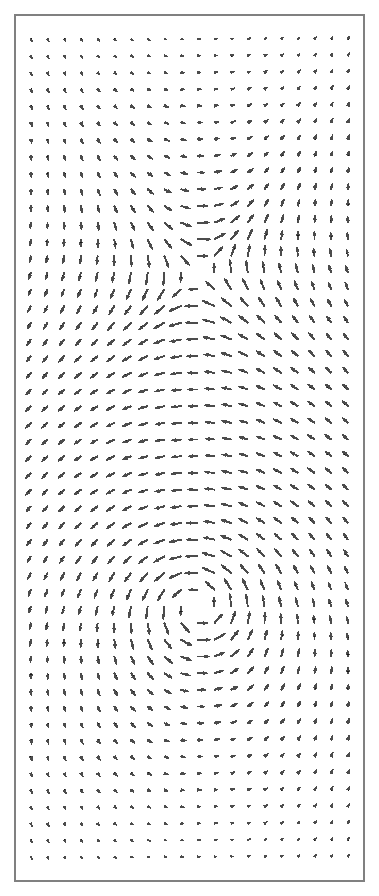
\includegraphics[width=0.5\textwidth]{figs/vortex.pdf}
	\begingroup
\setbox0=\hbox{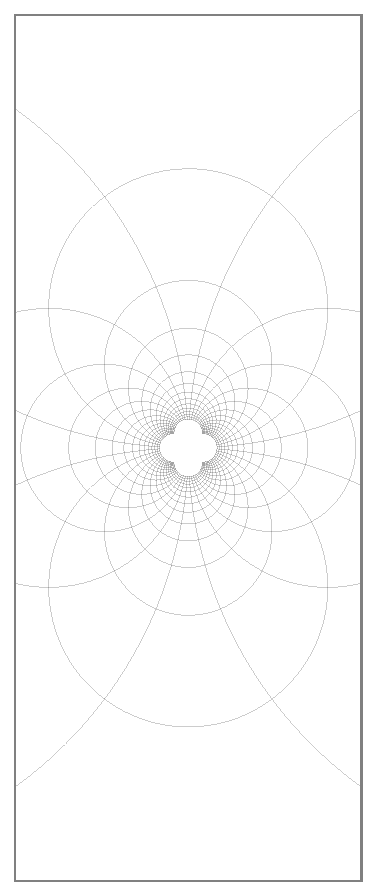
\includegraphics{fig/sct.pdf}}%
\parbox{\wd0}{\box0}\endgroup
\end{titlepage}

\dominitoc 
\tableofcontents

\chapter{January}
\begin{tocbox}
	\minitoc
\end{tocbox}

\entry{An Explicit Abelianization}{1/9/24}
\parhead{Dihedral group}
The simplest non-abelian group available is the dihedral group $ \text{D}_6
\simeq \mathbb{Z}_2 \ltimes \mathbb{Z}_3 $, the symmetry group of a triangle.
The $ \mathbb{Z}_2 $ consists of the reflection of the triangle, and the 
$ \mathbb{Z}_3 $ is the rotations by $ 2\pi / 3 $ degrees. Thus we have 
\begin{equation*}
	\text{D}_6 \simeq \left\{ e, r, r^2 \right\} \ltimes \left\{ e, p \right\}
\end{equation*}
It's not too hard to draw a bunch of triangles and find that this group has the 
following Cayley table:

\begin{table}[h]
\centering
\begin{tabular}{c | c c c c c}
		     & $ r $    & $ r^2 $  & $ p $    & $ rp $   & $ r^2 p $ \\ \hline
	$ r $    & $ r^2 $  & $ e $    & $ rp $   & $ r^2p $ & $ p $     \\
	$ r^2 $  & $ e $    & $ r $    & $ r^2p $ & $ p $    & $ rp $    \\ 
	$ p $    & $ r^2p $ & $ rp $   & $ e $    & $ r^2 $  & $ r $     \\ 
	$ rp $   & $ p $    & $ r^2p $ & $ r $    & $ e $    & $ r^2 $   \\
	$ r^2p $ & $ rp $   & $ p $    & $ r^2 $  &  $ r $   & $ e $
\end{tabular}
\end{table}

Here the nontrivial identities which require some toying around with the 
triangles are $ pr = r^2 p $, $ pr^2 p = r $, $ pr^2 = rp $.

\parhead{The semidirect} What is the semidirect product structure on $
\mathbb{Z}_2 $ and $ \mathbb{Z}_3 $ that produces $ \text{D}_6 $?
We can do this with a procedure identical to that which we performed on the 
$ \text{U}(1)\ltimes \mathbb{Z}_2 $ symmetry of the particle on a ring of the
2023 logs. Now, there are two identities that capture the non-commutativity 
of the two symmetries, $ pr^2p = r $ and $ prp  = r^2 $ (two comments: first, 
notice this is like $ PT_{\alpha} P = T_{-\alpha} $ for $ \text{U}(1)\ltimes
\mathbb{Z}_2 $, and also notice that these are precisely the commutators with 
$ p^{-1} = p $). We find 
\begin{align*}
	&pr^2 p = (p,e) \cdot (e, r^2)\cdot(p, e)
		= (p, e)\cdot(p, r^2 \varphi_e(e))
		= (p^2, \varphi_p(r^2))
		= (e, r)\\ 
	&prp = (p, e) \cdot (p, \varphi_p(r)) = (p^2, r^2) = (e, r^2)
\end{align*}
provided $ \varphi_p(r^2) = r $---we don't even have to require $ \varphi_p(r) = r^2 $ because there is no other choice in this automorphism of $ \mathbb{Z}_3 $.

\parhead{Commutator} The commutator subgroup $ [G, G] $ is the subgroup generated 
by the commutators of $ G $. If the group is abelian, the commutator subgroup 
is trivial. The commutator is $ [a,b] = a^{-1} b^{-1} a b$; indeed it measures how 
the conjugation by $ a $ changes $ b $ (or vice-versa): if $ a $ and $ b $
commute
\begin{equation*}
	[a,b] = e \quad \iff \quad a^{-1} b a = b.
\end{equation*}

\parhead{Abelianization} Let's compute the abelianization $ \text{D}_6 /
[\text{D}_6,\text{D}_6] $ by finding what $ [\text{D}_6, \text{D}_6] $ is. 
We have 
\begin{align*}
	[r, r^2] = e, \qquad [p, r] = prp^{-1} = prpr^2 = r^2 r^2 = r, \\ 
	[r, p] = rpr^2 p = r^2 ,\qquad [p, r^2] = pr^2 pr = r^2.
\end{align*}
Evidently $ r $ generates the commutator subgroup and we have that $
[\text{D}_6, \text{D}_6] \simeq \mathbb{Z}_3$ and thus the abelianization is 
\begin{equation*}
	\text{D}_6/[\text{D}_6, \text{D}_6] \simeq \mathbb{Z}_2,
\end{equation*}
which makes sense because when the group fails to commute the difference in the 
resulting actions is a rotation.


\entry{Central Charge and Second Cohomology}{1/15/24}
Blumenhagen and Plauschinn: 

\begin{quotebox}
Is is generally true that $ H^2(\mathfrak{g},\mathbb{C}) $ classifies the central 
extensions of an algebra $ \mathfrak{g} $ modulo redefinitions of the generators. 
However, for semi-simple finite dimensional Lie algebras, one finds that their
second cohomology group vanishes and so in this case there do not exist any
central extensions.
\end{quotebox}

\subsection{Group Cohomology}
Intuitively, group (co)homology can be be understood as
the (co)homology of the classifying space of the group $ G $, $ \mathrm{B}G $,
which is the space whose fundamental group is $ G $: $ \pi_1(\text{B}G) = G $
(the Eilenberg-MacLane theorem guarantees us such a space). 
For the purposes of
computation, however, we need a more concrete construction akin to a simplicial
complex structure on a topological space. 

TODO classifying space vs eilenberg maclane space?

\parhead{Simplicial resolution} The so-called \textbf{simplicial 
resolution}\footnote{For the present purposes, it suffices to think of a 
resolution as a chain complex; indeed it has the same structure as an exact 
sequence.} does the job in a fairly intuitive way: we think of elements of $ G $ 
as vertices in a simplex, with $ n $-simplices formed of $ n $-tuples of elements 
of $ G $, and consider the simplicial chain complex of this simplex. To be 
specific, 
\begin{equation*}
	C_n = \bigoplus_{G^{n+1}} \mathbb{Z}
\end{equation*}
whose basis elements are $ (g_0, \dots, g_n)\in G^n $, and with boundary map 
identical to that of simplicial complexes: 
\begin{align*}
	\partial_n C_n &\longrightarrow C_{n-1} \\ 
	(g_0, \dots, g_n) &\longmapsto \sum_{i = 0}^{n}(-1)^i (g_0, \dots, \hat{g}_i, \dots,g_n)
\end{align*}

\parhead{Bar resolution} An alternative resolution (which will come into play shortly) is the \textbf{bar
resolution} 
\begin{equation*}
	\bar{C}_n = \bigoplus_{G^n} \mathbb{Z}G
\end{equation*}
(the practical difference between this and the above direct sum is not manifest to me) 
whose basis elements are denoted $ [g_1\vert g_2 \vert \cdots \vert g_n] $.
Here $ \mathbb{Z}G $ is a $ \mathbb{Z}G $-module---defined as an action of $ G $ 
on the abelian group $ \mathbb{Z} $ satisfying $ g(a + b) = ga + gb $, we can
think of elements of $ \mathbb{Z}G $-modules as simplicial chains in the sense
that 
\begin{equation*}
	g_1 n_1 + g_2 n_2 + \cdots + g_N n_N , \qquad n_i\in \Z
\end{equation*}
is in a $ \mathbb{Z}G $ module. This comes with its own boundary map 
\begin{align*}
	\bar{\partial}_n \bar{C}_n &\longrightarrow \bar{C}_{n-1} \\ 
	[g_1 \mid \cdots \mid g_n] &\longmapsto
	g_1 [g_2 \mid \cdots \mid g_n]\\
		&\qquad \qquad + \sum_{i = 1}^{n-1}(-1)^i [g_1\mid\cdots\mid g_{i-1} \mid g_i g_{i+1}\mid 
		g_{i+1} \mid \cdots \mid g_{n}]\\
		&\qquad \qquad + (-1)^n [g_1 \mid \cdots \mid g_{n-1}]
\end{align*}
\parhead{Equivalence of resolutions} (It is the corresponding coboundary map of
the bar boundary map that will appear in the classification of the central
extension). The two constructions can be related by a map 
\begin{equation*}
	[g_1 \mid \cdots \mid g_n] \mapsto 
	(e, g_1, g_1 g_2, \dots , g_1 g_2 \cdots g_n)
\end{equation*}
which actually is an isomorphism, meaning that the bar and simplicial resolutions 
are entirely isomorphic and their (co)homologies will agree. Actually, this is 
an instance of a broader fact---these resolutions are both \textbf{projective},
and all projective resolutions are chain homotopy equivalent $ \Longrightarrow  $
their (co)homologies agree.

\subsection{Central extensions from cohomology}
Consider the central extension $ \tilde{G} $ of $ G $ by $ Z $:
\begin{equation*}
	0 \longrightarrow 
	Z
	\longrightarrow
	\tilde{G}
	\longrightarrow
	G
	\longrightarrow 
	0
\end{equation*}
Now, to differentiate the abelian group composition of $ Z $ from the 
nonabelian composition of $ G $ and $ \tilde{G} $, we will write $ Z $ as the 
formal exponentiation of some additive abelian group $ Z = \exp(F) $. (This is
also in anticipation of the interpretation of $ Z $ as a phase in some field 
$ F $, e.g., $\R$.) 

We are guaranteed that $ G \simeq \tilde{G} / \exp(F)$, although this isomorphism 
is not canonical---one way you can think of this is we need to choose which
phase will go on each element of $ G $. To be formal,
$ \tilde{G} /\exp(F) = \{ \tilde{g} \exp(F) \mid \tilde{g}\in \tilde{G} \}$; 
the isomorphism assigns each element of $ g $ to a representative of a coset 
$ \tilde{g}\exp(F) $ (i.e., an arbitrary element of that coset, meaning an element 
of $ \tilde{g} $ with some phase); such a set---one composed of a representative 
from each coset---is termed a \textit{section}. 

At any rate, having made such a choice, the isomorphism is canonical. Let it be 
$ \gamma : G \to \tilde{G}/Z $. Then every element of $ \tilde{G} $ can be written 
as some $ \gamma(g)\exp(a) $, $ g\in G $, $ a\in F $, and the composition 
is generally 
\begin{equation}\label{eq:group-cohom-composition}
	\gamma(g_1)\gamma(g_2) = \gamma(g_1 g_2) \exp(c(g_1, g_2))
\end{equation}
with $ c $ some function $ G\times G \to F $.
Now, generally functions $ G^n \to F $ are group $ n $-cochains (strictly speaking 
$ F $ needs to be a $ G $-module, though I'm not sure how $ G $ acts on $ F $
in this case), so $ c $ is a group 2-cochains, but not one that is uniquely 
determined by $ \tilde{G} $. Specifically, we can choose another section, say 
$ \gamma' $, under which 
\begin{equation}\label{eq:group-cohom-composition-prime}
	\gamma'(g_1)\gamma'(g_2) = \gamma'(g_1 g_2) \exp(c'(g_1, g_2))
\end{equation}
Now, in transforming to our original section $ \gamma $ the worst that can 
happen is we acquire a phase: 
\begin{equation*}
	\gamma'(g) = \gamma(g) \exp(d(g))
\end{equation*}
for some $ d : G \to F $. Then we have \cref{eq:group-cohom-composition-prime} 
becomes 
\begin{align*}
	\gamma(g_1) \exp(d(g_1))\gamma(g_2)\exp(d (g_2)) &= \gamma(g_1 g_2) 
		\exp(d(g_1 g_2)) \exp(c'(g_1, g_2))\\ 
	\gamma(g_1) \gamma(g_2) &= \gamma(g_1 g_2) \exp\left[
		d(g_1 g_2) - d(g_1) - d(g_1) + c'(g_1, g_2)
	\right]
\end{align*}
Comparing with \cref{eq:group-cohom-composition} we find 
\begin{equation*}
	c(g_1, g_2) - c'(g_1, g_2) = d(b_1 b_2) - d(b_1) - d(b_2) 
\end{equation*}
The right hand side is nothing but the (bar) coboundary map $ \delta d(b_1, b_2) $, 
so we have found that that any two central extensions are determined only up to a 
coboundary.

On the other hand, consider the following composition: 
\begin{align*}
	\gamma(g_1) \gamma(g_2) \gamma(g_3) &= \gamma(g_1 g_2) \gamma(g_3) \exp(c(g_1, g_2))\\
		&= \gamma(g_1 g_2 g_3) \exp(c(g_1, g_2)) \exp(c(g_1 g_2, g_3))
\end{align*}
But associativity tells us
\begin{align*}
	\gamma(g_1) \gamma(g_2) \gamma(g_3) &= \gamma(g_1) \gamma(g_2 g_3) \exp(c(g_1, g_2))\\
		&= \gamma(g_1 g_2 g_3) \exp(c(g_2, g_3)) \exp(c(g_1, g_2 g_3))
\end{align*}
Equating the two right hand sides:
\begin{align*}
	&\gamma(g_1 g_2 g_3\exp(c(g_1, g_2)) \exp(c(g_1 g_2, g_3)))
		= \gamma(g_1 g_2 g_3) \exp(c(g_2, g_3)) \exp(c(g_1, g_2 g_3))\\
	&\qquad \Longrightarrow \exp(c(g_1, g_2) + c(g_1 g_2, g_3) - c(g_2 , g_3) - c(g_1, g_2 g_3)) = 1\\ 
	&\qquad \Longrightarrow  c(g_1, g_2) + c(g_1 g_2, g_3) - c(g_2 , g_3) - c(g_1, g_2 g_3) = 0
\end{align*}
again, this is in fact nothing but the coboundary map $ \delta c(g_1, g_2, g_3) $, 
so that $ c $ is in fact a cocycle (it has vanishing coboundary). 

\parhead{Cohomology} What we've learned is that the central extension is
determined by a 2-cocycle $ c $ up to the addition of a 2-coboundary $ d $, thus
it is classified by the second group cohomology $ H^2(G, F) = \ker \delta /
\text{im}\, \delta$.
Now, the remarkable fact is that this is also the case at the level of the Lie 
algebra---the central extensions (properly, the central charge) is classified 
by the second Lie algebra cohomology $ H^2(\mathfrak{g}) $. We can also
understand this by noticing that the central charge is nothing more than the
generator of $ Z $---it is the generator of the central extension, hence the
terminology ``central charge'' (it is the generator---the charge---of the
center). It is a consequence of the Whitehead lemma that $ H^2(\mathfrak{g}) = 0$
if $ \mathfrak{g} $ is semisimple, meaning the semisimple Lie algebras cannot 
carry a central charge.

Here is a quick illustration of how the above considerations play with 
central charges as they appear at the level of the algbera. Provided $ [X,Y] $ is central, 
\begin{align*}
	e^X e^Y e^{-X} e^{-Y}
		&= e^{X + Y + \frac{1}{2}[X,Y]} e^{-X} e^{-Y}\\
		&= e^{X + Y  + \frac{1}{2} [X,Y] - X + \tfrac{1}{2} [X, Y + \frac{1}{2}[X,Y], -X]} e^{-Y}\\
		&= e^{Y + \frac{1}{2}[X,Y] - \frac{1}{2}[Y,X]} e^{-Y}\\ 
		&= e^{Y + [X, Y] -Y + \cancel{ \frac{1}{2} [[X,Y], Y]}}\\ 
		&= e^{[X,Y]}
\end{align*}
(this is a neat formula relating the algebra commutator to the group commutator). 
Then
\begin{align*}
	e^{\gamma([X,Y])} &= \gamma(e^{X}) \gamma(e^Y)\gamma(e^{-X}) \gamma(e^{-Y})\\
		&= \gamma(e^X e^Y e^{-X} e^{-Y})
			e^{c(e^X, e^Y)}
			e^{c(e^X e^Y, e^{-X})}
			e^{c(e^X e^Y e^{-X}, e^{-Y})}\\
		&= \gamma(e^{[X,Y]}) e^{C(X,Y)}
\end{align*}
Then 
\begin{equation*}
	\gamma([X,Y]) = [X,Y] + C(X,Y)
\end{equation*}

\subsection*{References} 
\begin{itemize}[nosep]
\item Clara L\"oh, \href{https://loeh.app.uni-regensburg.de/teaching/grouphom_ss19/lecture_notes.pdf}{Group Cohomology}.
\item user568976, Understanding the relation between central extensions and
	2-cocycles and coboundaries, URL (version: 2020-04-17):
	\url{https://math.stackexchange.com/q/3629722}
\end{itemize}


% \entry{Lessons from software engineering}{1/19/24}
% It just occurred to me that I've made a good amount of growth as a physicist by 
% transplanting some of the habits I built in software engineering. Specifically: 
% Part of what drew me to computational work in the first place was a certain 
% convenience that it afforded---computers do the tedious work and leave the fun 
% parts to you, and even if it takes many hours and tears, once you write a
% program that does that tedious work you can easily (1) clean it up and optimize,
% and (2) reuse the code, assured that for the most part it is set in
% stone. 

% The point is that your pen-and-paper calculations can improve by borrowing from 
% this mindset. This manifests as a slight change in mental and practical
% approach: 
% \begin{itemize}[itemsep=0pt, topsep=0pt]
% \item Be a compulsive notetaker and keep those notes neat, organized, and correct.
% 	Thoroughness and clarity is analogous to good code documentation. Don't be 
% 	afraid to return to the work and clean it up.
% \item Treat calculations others have done as ``code'' you can adapt to your own 
% 	problems. 
% \end{itemize}
% Here's the motivating example: while at the airport terminal, vacantly staring at 
% the above Cayley table for $ \text{D}_6 $, I realized that if I ever need 
% to work out any other constructions defined on a non-abelian group, I already 
% understand $ \text{D}_6 $ relatively well, and could reuse the above work. Thus
% that entry is sort of like ``code'' that's written and available
% to be reused; by being thorough about its correctness I will be sure that those
% usages are less foolproof.  Having toy examples and models is crucial in
% physics, and understanding one 
% toy model well that is capable of conveying many phenomena is not only a useful 
% exercise, but one that can be built on in the future.

%%%%%%%%%%%%%%%%%%%%%%%%%%%%%%%%%%%%%%%%%%%%%%%%%%%%%%%%%%%%%%%%%%%%%%%%%%%%%%%%
%%%%%%%%%%%%%%%%%%%%%%%%%%%%%%%%%%%%%%%%%%%%%%%%%%%%%%%%%%%%%%%%%%%%%%%%%%%%%%%%

\chapter{February}
\begin{tocbox}
	\minitoc
\end{tocbox}

\entry{QFTs from Neural Networks}{2/1/24}
In QFT topological defects are fixed points of RG flow---if learning is like an 
rg flow, what happens if there's a topological defect in a NN?

\entry{Chern-Simons Theory}{2/5/24}
Here's a silly mnemonic to remember the Chern-Simons term: the godmother of 
computing, Ada Lovelace, was inspired by the mechanism of mechanical looms,
which performed weaves and braids not unlike those of the anyons that populate 
a Chern-Simons theory. The term $ A\wedge \text{d} A $, is associated as 
$ A\wedge \text{d}A \rightarrow \text{AdA} \rightarrow \text{Ada Lovelace} $. 

(What's that? Doesn't the wedge product of any form with itself vanish? No, silly, 
recall these are \textit{Lie algebra-valued one forms}, for which the wedge product 
is essentially the commutator. If this theory was Abelian, however, the wedges 
\textit{would} vanish.)

\subsection{Anyons in the semiclassical theory}
\begin{equation*}
	\mathcal{L}
		= \frac{k}{4\pi} \epsilon^{\mu\nu\rho} A_\mu \partial_\nu A_\rho
			+ A_\mu J^\mu
\end{equation*}
\begin{equation*}
	\frac{\delta S}{\delta A_\mu}
		= 0 \Longrightarrow 
		0 = \frac{k}{4\pi}\epsilon^{\mu\nu\rho} \partial_\nu A_\rho + J^\mu
		\Longrightarrow  
		\frac{k}{4\pi} \epsilon^{\mu\nu\rho} \partial_\nu A_\rho = -J^\mu
\end{equation*}
\begin{align*}
	\frac{k}{4\pi} \epsilon^{ij}\partial_i A_j = J^0 = \rho 
	&\Longrightarrow \frac{k}{2\pi} B = \rho\\ 
	\frac{k}{4\pi} \epsilon^{ij} (\partial_j A_0 - \partial_0 A_j)
		= -J^i 
	&\Longrightarrow \frac{k}{4\pi}\epsilon^{ij} E_j = J^i
\end{align*}

The Wilson lines obey the algebra 
\begin{equation*}
	W_x W_y = e^{2\pi i / k} W_y W_x
\end{equation*}
But note that this implies $ W_y^k $ commutes with $ W_x $:
\begin{equation*}
	W_x W_y^k = (e^{2\pi i / k})^k W_y^k W_x
		\Longrightarrow W_x W_y^k  = W_y^k W_x
\end{equation*}
and, of course, $ W_y^k $ commutes with any power of $ W_y $, so $ W_y^k $ is 
in the center, which by Schur's lemma implies that it is proportional to the 
identity. It is the Casimir of this algebra

Now consider some state $ \ket{n} $ in this representation labelled by quantum 
number $ n $ so that $ W_x\ket{n} = \lambda_n \ket{n} $. Then
\begin{equation*}
	W_x W_y \ket{n} = e^{2\pi i / k} W_y W_x \ket{n} 
		= e^{2\pi i / k} W_y \lambda_n \ket{n} 
		= e^{2\pi i/ k}\lambda_n W_y \ket{n}
\end{equation*}
So $ W_y\ket{n} $ has eigenvalue $ e^{2\pi i / k}\lambda_n \ket{n} $ and $ W_y $
acts as a raising operator. But $ W_y^k = 1 $, so one can only move up in the 
weight lattice $ N $ times. Thus we have a $ k $-dimensional irrep, and a 
$ k $-degenerate groundstate. In fact, this is the irrep of the $ 1 $-form 
symmetry generated by the Wilson lines CS theory enjoys.


\subsection{Large-\textit{k} partition function and framing anomaly}
We study the nonabelian Chern-Simons partition function at large $ k $, following 
Witten (1989) and Witten and Bar-Natan (1991). Analogous to the large-$ N $
approximation, large-$ k $ Chern-Simons theory justifies approximating the 
partition function by its saddle-point---i.e., its classical equation of motion. 
Since for Chern-Simons theory this equation of motion is $ F^{{\mu\nu}} = 0 $, 
the saddle-point corresponds to the ``\textit{moduli space}'' of flat
connections.\footnote{Physicists can think of moduli spaces as the space of
configurations satisfying a certain requirement.}
\begin{align*}
	(A^{(\alpha)} + a) \wedge \text{d}(A^{(\alpha)} + a)
		= A^{(\alpha)} \wedge \text{d}A^{(\alpha)} + A^{(\alpha)} \wedge \text{d}a 
			+ a\wedge \text{d}A^{(\alpha)} + a\wedge \text{d}a
\end{align*}
(temporarily suppressing the $ (\alpha) $ index)
\begin{align*}
	(A + a) \wedge (A + a) \wedge (A + a) 
		&= (A + a) \wedge \left[
			A \wedge A + A \wedge a + a \wedge A + a \wedge a
		\right] \\ 
		&= A \wedge A \wedge A 
			+ A \wedge A \wedge a 
			+ A \wedge a \wedge A 
			+ A \wedge a \wedge a \\
		&\qquad + a \wedge A \wedge A 
			+ a \wedge A \wedge a 
			+ a \wedge a \wedge A 
			+ a \wedge a \wedge a
\end{align*}
Treating $ a $ as small, we ignore the third-order term
\begin{align*}
	&= A \wedge A \wedge A 
				+ \cancel{A \wedge A \wedge a}
				+ A \wedge a \wedge A 
				+ \cancel{A \wedge a \wedge a} \\
			&\qquad + \cancel{a \wedge A \wedge A}
				+ a \wedge A \wedge a 
				+ \cancel{a \wedge a \wedge A }
\end{align*}
The indicated terms cancel because for the wedge product of Lie algebra-valued 
forms we have 
\begin{equation*}
	\alpha\wedge\beta = (-1)^{1 + \deg a\cdot \deg \beta} \beta\wedge \alpha
\end{equation*}
and recall that since we are expanding about the saddle-point, linear fluctuations 
vanish and we have
\begin{align*}
	&= A \wedge A \wedge A 
				+ a \wedge A \wedge a 
\end{align*}
Thus we are left with 
\begin{align*}
	\mathcal{L} &= A^{(\alpha)} \wedge \text{d} A^{(\alpha)}
					+ A^{(\alpha)} \wedge A^{(\alpha)} \wedge A^{(\alpha)}
					+ a\wedge(\text{d}a + A^{(\alpha)} \wedge a)\\ 
				&= \mathcal{L}_{\text{CS}}[A^{(\alpha)}]	
					+  a\wedge Da
				= \mathcal{L}_{\text{CS}}[A^{(\alpha)}]	
					+ \epsilon^{\mu\nu\rho} a_\mu D_{\nu} a_\rho
\end{align*}
where we've identified a covariant derivative for the saddle point field 
configuration $ D = \text{d} + A \wedge \cdot = \partial_\mu + [A_\mu,\cdot]$.

Now, we introduce the \textit{elliptical operator} $ \star D + D\star $. This 
operator manifestly maps odd-degree forms to odd-degree forms and even-degree 
forms to even-degree forms, so one can consider its action on the space of 
odd forms strictly, which we call $ L_- $. In three-dimensions $ L_- $ acts 
on $ \Omega^1(M) \oplus \Omega^3 (M) $; we thus combine $ (a,\phi) $ into an 
element of $ \Omega^1(M) \oplus \Omega^3 (M) $ and observe that then 
\begin{align*}
	(a,\phi) \wedge \star (\star D + D \star) (a,\phi)
		&= (a,\phi) \wedge \star (\star D a + D\star \phi, \cancel{\star D \phi} + D\star a )\\
		&= a \wedge D a + \cancel{a \wedge \star D \star \phi} + \phi \star D\star a 
\end{align*}
(Notice that $ L_- $'s action is a bit subtle here---we get mixing of components 
in the sense that $ a \in \Omega^1 $ but $ D\star a \in \Omega^3 $, so we must 
take it to the second component.) The indicated term vanishes in the last 
line because $ \phi $ is non-dynamical. Also, if $ \phi\star D\star a $ looks 
suspicious, notice that $ \star D \star a $ is a zero form, i.e., a scalar, 
so this is just scalar multiplication on $ \phi $.


\subsection{1-form symmetry}

\subsection{Spin manifolds}
Consider integration by parts for forms: 
\begin{equation*}
	\int_X d\alpha \wedge \beta = \int_X \left[d(\alpha\wedge\beta) 
		- (-1)^{\deg \alpha}\alpha\wedge d\beta\right]
		= \int_{\partial X}\alpha\wedge\beta 
			-(-1)^{\deg \alpha} \int_{X}\alpha \wedge d\beta
\end{equation*}
Thus setting $ \alpha = A $ and $ \beta = dA $, one finds 
\begin{equation*}
	\int_X F \wedge F 
		= \int_{\partial X} A \wedge dA
	-(-1)^{\deg\alpha}\int_{X} \cancel{A \wedge d^2 A}
\end{equation*}
The argument is that for this extension to be consistent, the partition function 
needs to be the same for any two $ X_1 $ and $ X_2 $ sharing $ M $ as a boundary. 
Thus, we may glue two such $ X_1 $ and $ X_2 $ along $ M $ (so that the integral 
becomes an integration over $ Y $ the manifold resulting from the gluing): 
\begin{equation*}
	\Delta S_{\text{CS}}
		= S_{\text{CS}}^{X_1}
		  - S_{\text{CS}}^{X_1}
		= \frac{k}{2\pi}\int_Y F\wedge F
\end{equation*}
If we stipulate 
\begin{equation*}
	\frac{k}{4\pi} \int_Y F\wedge F
		\in 2\pi\mathbb{Z}
		\iff 
	\frac{k}{8\pi^2} \int_Y F\wedge F
		\in \mathbb{Z}
\end{equation*}
we have $ e^{\Delta S_{\text{CS}}} = e^{i2\pi n}= 1$ and the partition function 
is invariant. When is the above true? As it turns out, exactly when $ Y $ is a 
spin manifold, which leads to the integral resolving to an integer
\begin{equation*}
	\int_Y F\wedge F \in 2\mathbb{Z} \Longrightarrow  \Delta S_{\text{CS}} = 
	2\pi k \cdot n \in 2\pi \mathbb{Z}
\end{equation*}

When $ Y $ does not meet this condition, the integral is simply an integer
\begin{equation*}
	\int_T F\wedge F \in \mathbb{Z} \Longrightarrow \Delta S_{\text{CS}} =
	2\pi k \cdot \frac{n}{2} \in 2\pi \mathbb{Z}
	\text{ only if }k\in 2\mathbb{Z}
\end{equation*}
i.e., the Chern-Simons level must be \textit{even} in addition to being an 
integer.

How could this possibly be true? First things first: here we can view 
$ F /2\pi $ as a member of $ H^2(Y;\mathbb{Z}) $. $ dF = 0 $ by the Levi-Civita 
identity---i.e., because $ F = dA $---so it is in the kernel of the coboundary 
map, and in this context 
\begin{align*}
	(F+ d\alpha)\wedge (F+ d\alpha)
		&= F\wedge F 
			+ d\alpha \wedge F + F\wedge d\alpha
			+ d\alpha\wedge d\alpha\\
		&= F\wedge F + d^2\alpha \wedge \alpha 
			+ \underbrace{\cancel{2 d(\alpha \wedge F) + d(\alpha \wedge d\alpha)}}_{\text{no }\partial X}
\end{align*}
so it is only defined up to an exact form. Lastly, $ F/2\pi \in H^2(Y, \mathbb{Z}) $
because the integral of $ F $  is valued in $ 2\pi \mathbb{Z} $ thanks to the 
Dirac quantization condition. Recall that in this case elements of the
cohomology implicitly come up with an integration---this is the appropriate
approach for differential cohomology, for instance De Rham cohomology.
Correspondingly, cup products turn into wedge products.

We can make contact with the Stiefel-Whitney class, we consider the reduction
\begin{equation*}
	H^2(Y;\mathbb{Z}) \to H^2(Y;\mathbb{Z}_2)
\end{equation*}
so the lift of the Stiefel-Whitney class $ w_2 $ is only defined mod 2. For 
instance $ w_2 $ vanishing corresponds to it being even valued in $
H^2(Y;\mathbb{Z}) $. Additionally, the intersection form satisfies 
\begin{equation*}
	\frac{F}{2\pi}\smallsmile \frac{F}{2\pi} = w_2 \smallsmile \frac{F}{2\pi}
\end{equation*}
(TODO why is this true?). Since $ F/2\pi\in\mathbb{Z} $ and $ w_2 \in 2\mathbb{Z}$ 
if the manifold is spin, one has the intersection form is an even integer, and 
\begin{equation*}
	\int_Y \frac{F}{2\pi} \wedge \frac{F}{2\pi} \in 2\mathbb{Z}
\end{equation*}
and when the manifold is not spin, it is simply integer-valued.

\subsection*{References}
\begin{itemize}[nosep]
\item Sachdev, ``Topology and Chern-Simons Theories,''
	\href{http://qpt.physics.harvard.edu/phys268/}{PHYS268}.
\item Witten, ``\href{https://projecteuclid.org/journals/communications-in-mathematical-physics/volume-141/issue-2/Perturbative-expansion-of-Chern-Simons-theory-with-noncompact-gauge-group/cmp/1104248307.full}{Perturbative expansion of Chern-Simons theory with noncompact gauge group}.''
\item Witten, ``\href{https://projecteuclid.org/journals/communications-in-mathematical-physics/volume-121/issue-3/Quantum-field-theory-and-the-Jones-polynomial/cmp/1104178138.full}{Quantum Field Theory and the Jones Polynomial}.''
\item Ethan Lake, \href{https://drive.google.com/file/d/1wNJaNX1Ef1hrOly-TET8yKG2rx7mcaH0/view}{\textit{QFT Diary}}.
\item Santiago Quintero de los R\'ios
``\href{https://webspace.science.uu.nl/~caval101/homepage/Students_files/QuinteroMaster.pdf}{Seiberg-Witten
Theory and the Intersection Form}''
\end{itemize}

\entry{Spin Manifold Miscellany}{2/11/24}
\subsection{Vierbeins, Tetrads, Spin Connections}
The vierbein (German for ``four-legged'') formalism is an alternative formulation
of a coordinate system on a curved manifold which is intimately related to the
spin connection. They are defined as the eigenvalues of the metric: 
\begin{equation*}
	g_{\mu\nu} = e_\mu^a (x) \eta_{ab} e_{\nu}^{b}(x)
\end{equation*}
Notice that, viewing the metric as a background field, the vierbein formalism 
essentially defines a field $ e^{a}_\mu(x) $, which we interpret as the (local)
coefficients for a vector expressed in a \textit{fixed} orthonormal basis 
(referred to as the \textbf{tetrad} basis). 

Now, the more formal way to define the spin connection is as follows: There is a 
short exact sequence 
\begin{equation}\label{eq:spin-les}
	0 \longrightarrow \Z_2 \xrightarrow{\quad}
	\text{Spin}(N) \xrightarrow{\;\phi\;} \text{SO}(N) \longrightarrow 0
	\footnote{This is silly, but for a long time I wondered why we used 
	$\text{Spin}(N)$ instead of $\text{SU}(N)$ for spinors. Well, this only 
	holds for $N=3$, where $\text{Spin}(3) \simeq \text{SU}(2)$. On the other hand 
	$\text{Spin}(4)\simeq \text{SU}(2)\times \text{SU}(2)$, hence the two Weyl 
	spinors in relativistic theories.}
\end{equation}
which restates the familiar mantra ``spinors are the square root of vectors.''
Now, we might consider a $\text{Spin}(N)$ spin bundle related to an $ \text{SO}(N) $ 
vector bundle by $ \phi $.
Where the Levi-Civita connection is the connection appropriate for vectors---i.e., 
it can be thought of as an $ \text{SO}(N) $ action---the spin-connection is the 
connection on spinors $\in\text{Spin}(N)$ induced by the pullback of $ \phi $. 
To be sure that everything is well defined, there is a Levi-Civita one form 
\begin{equation*}
	\omega_{ij}(X) = g(\del_X e_i, e_j) \qquad(\text{corresponding to }D_\mu)
\end{equation*}
the pullback $\phi^\ast \omega$ of which is the spin connection.
In this construction $ N $ is the dimension of the manifold (since $ \text{SO}(N) $)
is the structure group of the orthonormal frame bundle, which seems to place
some constraints on the spinor bundle $ \text{Spin}(N) $ that you can put on the
manifold (though maybe you can fiber $ N>\dim M $ bundles on it through an
immersion?).

Another way to think of why we might need the spin connection: as it turns out, 
there are no finite-dimensional spinor representations of the general covariance, 
or autoisometry group $ \text{GL}_4(\R) $ (LOOK INTO THIS) that gravity enjoys
as a symmetry. (Some authors refer to this as the diffeomorphism group, but they
are WRONG! See \cref{sec:diffeo-kerfuffle}.)
Since we know that the Lorentz group admits spinor representations, the trick 
is to extract the curvature of the manifold into the tetrad basis $ e^{\mu}_a(x) $, 
leaving behind the ``internal'' flat metric $ \eta_{ab} $ which of course 
transforms under the Lorentz group, thus allowing us to define spinorial
transformations in a curved spacetime according to the covariant derivative: 
\begin{equation*}
	D_\mu = \partial_\mu - \frac{i}{4}\omega_\mu^{ab} \sigma_{ab},\qquad 
	\sigma_{ab} = \frac{i}{2}\left[\gamma^a, \gamma^b\right]
\end{equation*}
and the spin connection is 
\begin{equation*}
	\omega_{\mu b}^a = e_\nu^a e_b^\lambda \Gamma_{\mu\lambda}^\nu
		- e_b^\lambda \partial_\mu e_\lambda^a.
\end{equation*}
This is the covariant derivative that would appear in, e.g., the Dirac 
equation on a curved background.

\subsection{Spinor Reps of GL\textsubscript{4}}
TODO

\subsection{Stiefel-Whitney classes}
Characteristic classes measure how bundles over a manifold twist, i.e., they 
measure obstructions to a global trivialization.
For a manifold $ M $, the class $ c $ associates an element of the 
cohomology $ c(P)\in H^k(M) $ to a given $ G $-bundle $ P $ (properly we should 
consider $ P $ a representative of an isomorphism class of $ G $-bundles). 
The characteristic class that measures obstructions to our ability to define
global orthonormal frame over the manifold is the first Stiefel-Whitney class.
Put it simpler terms, the first Stiefel-Whitney class measures the failure of
the manifold to be orientable.

Analogously, the second Stiefel-Whitney class measures the failure of a manifold 
to admit a spin structure, that is, a manifold is a spin manifold iff its second
Stiefel-Whitney class is trivial. We will see how much like how $ \text{Spin}(M) $
is the double cover of $ \text{SO}(M) $, the second Stiefel-Whitney class is 
sort of the double cover of the first.

\parhead{1st SW class} The first Stiefel-Whitney class is defined as the 
determinant of the transition maps on the charts of the manifold. Consider two
charts $ U_i $ and $ U_j $ related by the transition map $ t_{ij} $, itself a
member of the structure group $ \text{SO}(m =\dim M) $. ($ i $, $ j $ here do
not index the entries of the matrix but instead label the charts.) We define a $
1 $-cochain with coefficients in $ \mathbb{Z}_2 $ by the determinant of the
transition function: 
\begin{equation*}
	f(i,j)\equiv \det(t_{ij})  = \pm 1\qquad f\in C^1(M, \mathbb{Z}_2)
\end{equation*}
(This is a \v{C}ech cocycle). Now, $ t_{ij}t_{jk}t_{ji} = 1 $ because this 
transitions us back to the first chart $ i $. Consequently the coboundary map 
sends 
\begin{equation*}
	(\delta f)(i,j,k) = \det t_{ij}  \det t_{jk}  \det t_{ki}
		= \det(t_{ij} t_{jk} t_{ki}) = 1
\end{equation*}
And, further, if we consider transforming to a different frame on $ U_i $ 
by $ h_i \in \text{O}(m)$---and likewise for $ U_j $---the transition functions 
transform to $ t_{ij}\rightarrow h_i t_{ij} h_j^{-1}$, in which case we find 
\begin{equation*}
	f(i,j) \rightarrow \det(h_i t_{ij} h_j^{-1}) = 
	\underbrace{\det h_i \det h_j}_{\equiv (\delta f_0)(i,j)}
	\det f_{ij}
\end{equation*}
Here we've defined $ f_0(i) = \det h_i $ to be a $ 0 $-cochain. Thus 
$ f $ transforms by an exact $ 1 $-chain (which vanishes upon taking the 
coboundary map), and the equivalence class $ [f] $ of $ f $ up to a $0$-coboundary 
is evidently a member of $ H^1(M;\mathbb{Z}_2) $. This is the Stiefel-Whitney 
class, $w_1(M)=[f]$. 

\begin{barbox}[1st SW and Orientability]{mygreen}
	Now, the first Stiefel-Whitney class is trivial---all functions in $ [f] $ 
	are identically $ 1 $---iff the manifold is orientable. If $ M $ is orientable 
	the structure group is $ \text{SO}(m) $ and $ \det(t_{ij}) $ is necessarily
	unity. Meanwhile, if $ w_1(M) = 1 $, $ f(i,j) = (\delta f_0)(i,j) $ and we can 
	always choose $ h_i $ and $ h_j $ such that this product is unity (i.e., the 
	transition map continues to posses unit determinant).
\end{barbox}

\parhead{2nd SW class} The second Stiefel-Whitney class measures a slightly different obstruction: instead 
of taking the consistency of the transition maps for granted (and thus taking
the existentence of a tangent bundle for granted) and measuring their 
failure to preserve orientation as the first class does, the second measures the
failure of the transition maps to be consistent in the first place.
This is the sense in which it tells us whether we can put a consistent spin 
structure on the manifold. 

Consider the lift of $ t_{ij}\in \text{SO}(m) $ to
the double cover $ \tilde{t}_{ij} \in \text{Spin}(m)$, i.e., $ \tilde{t}_{ij} $
such that $ \phi(\tilde{t}_ij) = t_{ij}$ for the two-to-one homomorphism given
in \cref{eq:spin-les}. We of course need 
\begin{equation*}
	\tilde{t}_{ij}\tilde{t}_{jk}\tilde{t}_{ki} = I
\end{equation*}
for the spin bundle to be well-defined. We naturally also have 
\begin{equation*}
	\phi(\tilde{t}_{ij}\tilde{t}_{jk}\tilde{t}_{ki}) 
	= t_{ij} t_{jk} t_{ki}
	= I
\end{equation*}
Given the above and \cref{eq:spin-les}, $ \tilde{t}_{ij}\tilde{t}_{jk}\tilde{t}_{ki} $ 
can only fail to be the identity up to a multiplicative constant---in fact, it 
can only fail to be the identity up to a sign. Thus, we define 
a 3-cochain $ f $ satisfying
\begin{equation*}
	\tilde{t}_{ij}\tilde{t}_{jk}\tilde{t}_{ki}
		= f(i,j,k)I
\end{equation*}
Further, consider the two-cochain defined as the sign of the transition 
function $ \tilde{t}_{ij} $. Consider picking an arbitrary primage of $ \phi(t_{ij}) $
that might have a sign in front of it. Then we generalize to 
\begin{equation*}
	\tilde{t}_{ij}\tilde{t}_{jk}\tilde{t}_{ki}
	= f(i,j,k) I 
	\to 
	\underbrace{\sign(t_{ij})\sign(t_{jk})\sign(t_{ki})}_{(\delta f)(i,j,k)}
		f(i,j,k) I.
\end{equation*}
Thus $ f $ represents an equivalence class $ [f] \in H^2(M; \mathbb{Z}_2) $.

\begin{barbox}[2nd SW and Spin Structures]{mygreen}
Of course if the manifold is spin, $\tilde{t}_{ij}\tilde{t}_{jk}\tilde{t}_{ki}=1$, 
so $ w_2 $ is trivial. Converesely, if $ w_2 $ is trivial, it is defined up 
to a transformation 
\begin{equation*}
	\tilde{t}_{ij}\tilde{t}_{jk}\tilde{t}_{ki}
	\to 
	f(i,j) f(j,k) f(k,i) \tilde{t}_{ij}\tilde{t}_{jk}\tilde{t}_{ki}
\end{equation*}
But if $ f $ is trivial it is necessarily equal to $ (\delta f_1)(i,j, k) $, so we have 
\begin{equation*}
	\tilde{t}_{ij}\tilde{t}_{jk}\tilde{t}_{ki}
	\to 
	[f(i,j) f(j,k) f(k,i)]^2 I = I.
\end{equation*}
\end{barbox}

\subsection*{References}  
\begin{itemize}[itemsep=0.2ex]
\item Nakahara, \textit{Geometry, Topology and Physics} (2003), Section 11.6. 
\end{itemize}


$ O(n) \subset O(n+1) $. relative homotopy $ \pi_k(O(n+1), O(n)) \cong \pi_k(S^n)$.
$ \pi_k(A) \cong \pi_k(\tilde{A})  $ (generally true?).

Conformal anomaly relation to central charge

\entry{The Diffeomorphism Kerfuffle}{2/16/24}\label{sec:diffeo-kerfuffle}
People will commonly refer to general relativity theory as ``diffeomorphism 
invariant'' (or sometimes more inocuously, ``general covariant''), 
which they insist is euphemism for ``invariant wrt coordinate transformations.''
The culprit which motivated this entry was the claim that Chern-Simons theory is 
general covariant, but the framing anomaly breaks this covariance. Now, this 
case certainly helps to split the two notions---while gravity might be general 
covariant, it is certainly not diffeomorphism invariant in the sense that 
Chern-Simons theory is (independent of the metric and thus completely bendable). 

Ethan Lake comes to the rescue: ``...diffeomorphisms do not care about distances... 
such a theory would therefore need to be topological.'' He accuses the physics 
community of being terribly imprecise with terminology, and rightfully so:
what people refer to as \textit{diffeomorphism invariance} in fact refers to 
\textit{isometries}, transformations which preserve the metric (in a global 
sense that would also preserve its derivatives and thus the curvature) and thus 
the Einstein-Hilbert action; this is the \textit{true} symmetry of GR. To 
be explicit, an isometry $ f: (M,g) \to (N, h) $ has 
\begin{equation*}
	g(V,W) = h(f_\ast V, f_\ast W) 
	\iff 
	g_{\mu\nu} V^\mu W^\nu
		= h_{\alpha\beta} \frac{\partial y^{\alpha}}{\partial x^\mu}
			\frac{\partial y^\beta}{\partial x^\nu} V^\mu W^\nu
\end{equation*}
($ f_\ast $ being the pullback of $ f $). This means the metric transforms as 
\begin{equation*}
	h_{\alpha\beta}(y) = \left[ \frac{\partial y^{\alpha}}{\partial x^\mu}
			\frac{\partial y^\beta}{\partial x^\nu}\right]_{x} g_{\mu\nu}(x)
\end{equation*}
Properly, in GR we are concerned with what Lake calls ``autoisometries''---we 
are sending the manifold to itself. \textit{This} is the coordinate transformation 
people confuse for a diffeomorphism. We aren't changing the manifold, but 
generally change the metric by virtue of changing the coordinates.

WRITE A BIT ON THE KILLING EQUATION

\subsection*{References}
\begin{itemize}[nosep]
\item Ethan Lake,
\href{https://drive.google.com/file/d/1_w_JyW0Fppm94RNzSLckHALEUQ5xUHBH/view}{Manifesto
on spacetime symmetries, diffeomorphisms, and conformal transformations}.
\end{itemize}

\entry{Virtual Serial Ports for Development}{2/20/24}
I've been working on some software that reads a stream of bytes from a serial 
port---namely, an FPGA taking input from four photon detectors. The FPGA device 
is obviously not something I can take home; nonetheless, I want to be able to 
develop the software outside the lab. Naturally, what I need is a virtual serial port, 
which can be simulated with \mintinline{shell}{socat}:
\begin{minted}{shell}
socat -d -d pty,raw,echo=0 pty,raw,echo=0
\end{minted}

\entry{Anomaly: Fermion on a Ring}{2/20/24}
\subsection{'t Hooft Anomalies and Cohomology}

Homotopy $ \pi_k $ fails excision and additivity Eilenberg-Steenrod axioms. 

https://www.damtp.cam.ac.uk/user/tong/susy/susyqm2.pdf

\begin{itemize}
	\item Why $ T(m) = -m $. It's not that deep, just work it out in the action.
	$ \square $

	\item Explain how APS implies 
	\begin{equation*}
		\lim_{m \rightarrow \infty}
			\frac{Z[+m, g]}{Z[-m, g]} = \exp\left(i \int_X\text{CS}_\text{grav}\right)
	\end{equation*}

	Seems like something technical. In general look to understand the CS 
	gravity term, see if there's relation between the above and the fact that 
	it is the appropriate counterterm in the framing anomaly.

	\item How $ \rho(m) + \rho(-m) = 1 $? 
	\item Why $ Z[m] = 1 $ at long distances equiv to theory trivially gapped?
	My guess is that this amounts to ignoring spectra above a certain energy 
	scale, in which case there's just one state in the partition function. 
	\item Understand the whole ``nontrivial physics on interfaces'' bit.
\end{itemize}

\entry{Anomaly: Compact Boson}{...}

\entry{Landau Poles}{}

``Power divergence is strongest at the cutoff, logarithmic divergence receives 
equal contributions at all scales''
https://www.youtube.com/watch?v=RiMcxSz-PnI (13:52)

\entry{Zeta Function Regularization}{...}

GAMMAM MATRICES FLIP SIGN UNDER TIME REVERSAL

$ [Y, K(A,n)]\simeq H^n(Y,A) $ ($ K(A,n) $ is Eilenberg-Maclane space.)


%%%%%%%%%%%%%%%%%%%%%%%%%%%%%%%%%%%%%%%%%%%%%%%%%%%%%%%%%%%%%%%%%%%%%%%%%%%%%%%%
%%%%%%%%%%%%%%%%%%%%%%%%%%%%%%%%%%%%%%%%%%%%%%%%%%%%%%%%%%%%%%%%%%%%%%%%%%%%%%%%

\chapter{March}
\begin{tocbox}
	\minitoc
\end{tocbox}

\entry{Homotopy vs. Homology}{3/5/24}
Relationship between $ \pi_k $ and $ H_k $. $ H_1 $ is abelianization of $ \pi_1
$. In general the relationship is not so clear. E.g., $ \pi_2(\mathbb{R}\text{P}^2) 
= \mathbb{Z}$, $ H_2(\mathbb{R}\text{P}^2) = 0$. This is because
$\mathbb{R}\text{P}^2 = e^0\cup e^1 \cup e^2$ and 
\begin{equation*}
	\mathbb{Z}\left\{e^2 \right\} \xrightarrow[\partial]{2}
		\mathbb{Z}\left\{ e^1 \right\}\xrightarrow[\partial]{0} 
		\mathbb{Z}\left\{e^0\right\}
\end{equation*}
thus $ H_2(\mathbb{R}\text{P}^2)=0 $. (boundary of $ e^2 = 2e^1$).

Another example: $ X = \mathbb{C}\text{P}^\infty $ has 
\begin{align*}
	&H_k(X) = 
	\begin{cases}
	\mathbb{Z} & k\text{ even}\\
	0 & \text{else}
	\end{cases}\\
	&\pi_k(X) = \begin{cases}
	\mathbb{Z} & k=2\\
	0 & \text{else}
	\end{cases}
\end{align*}

\begin{enumerate}[itemsep=1pt]
\item Spaces that are weakly h.e. (in particular have the same $ \pi_k $) have 
	the same homology groups. Given $ f:X \to Y $ whe, wlog $ f: X \hookrightarrow Y $
	(mapping cylinder). WTS $ H_k(Y,X) \equiv 0 $, Fix $ [z] \in H_k(Y,X) $
	$ z=\sum a_i \sigma_i $ $ a_i \in \mathbb{Z} $, $ z $ cycle: $ \partial z \in 
	C_{k-1}(X)$, $ \sigma_i : \Delta^k \to Y $. Build complex $ (K,L) $ from $ z $
	$ \bigcup_i \Delta^k / \sim \partial $ $ K\subset \partial K $. (take two simplices 
	and glue along common boundary). By construction have map $ g:(K,L) \to (Y,X) $
	$ [w]\in H_k(K,L) $ s.t. $ g^\ast(w) = [z] $.  
	\begin{equation*}
		\begin{tikzcd}
		(K,L) \arrow[r] \arrow[dr, dashrightarrow]
		& (Y,X)\\
		& (X,X) \arrow[hook, u]
		\end{tikzcd}
	\end{equation*}
	Since $ H_k(X,X) = 0 $ this implies $ [z]=0 $. WTS $ (K,L)\to(Y,X) $
	homotopic to $ (K,L) \to (X,X) $. Use compression, $ \pi(Y,X) = 0 $
	to inductively construct homotopy as in proof of Whitehead.
\item If $ X $ is $ n $-connected ($ \pi_k=0 $ for $ k\leq n $)
	then also $ \tilde{H}_k=0 $ for $ k\leq n $. 
	Thm (cellular approx of spaces). Any space Z is whe to a cellular complex, 
	i.e.g,, $ \exists X $ cell complex and $ f:X \to Z $if $ Z $ is $ n $-connected 
	then can assume $X$ has no cells of dimensoin $ 1,\dots,n $. 
	Proof: $ X $ $ n $-connected. By cellular approx $ \exists Z $ cell complex 
	and whe $ Z\to X $ and $ Z $ has no cells in dim $ 1,\dots,n $. By 1.
	suffices to show $ \tilde{H}_k(Z) = 0 $, $ k\leq n $. 
	\begin{equation*}
		Z\left\{n+1\text{-cells}\right\}
		\to 0 \to \cdots \to 0\to\mathbb{Z}\left\{0\text{-cells}\right\}
	\end{equation*}
	using cellular homology $ \tilde{H}_k(Z)=0 $ $ k\leq w $. 
\item (Hurewicz) If $ X $ is $ n $-connected $ n\geq 2 $ then $ \pi_{n+1} (X)
\simeq H_{n+1}(X)$. 
\end{enumerate}



E.g., $ \mathbb{C}\text{P}^\infty $ 1-connected, $\pi_2(\mathbb{C}\text{P}^\infty) 
= H_2(\mathbb{C}\text{P}^\infty) $. 


\entry{assortment of spin chain facts}{...}
Shorter correlation length -> gapped
LSM. translational invariant so(3) interaction spin-1/2 chain is gapless. 
lieb-robinson bound 
gapless --- power law corr, gapped - exponential corr.

\entry{Fibrations}{3/9/24}
\parhead{Homotopy lifting property} A map between two spaces $ p : E \to B $ is
said to have the homotopy lifting property for a space $ X $, given a homotopy 
from $ X $ to $ B $ $ h:X\times[0,1] \to B $ and a lift $ \tilde{h}_0 : X \to E $ 
lifting the starting point of the homotopy $ h(0) \equiv h_0 $ (i.e., $ h_0 = 
p\circ \tilde{h}_0 $), there exists a homotopy $ \tilde{h} : X\times [0,1] \to E $ 
lifting $ h $ with $\tilde{h}(0) = \tilde{h}_0$. Diagrammatically:
\begin{equation*}
	\begin{tikzcd}
	X\times \left\{0\right\} \arrow[r, "\tilde{h}_0"] \arrow[d]
		& E \arrow[d, "p"] \\
	X\times\left[0, 1\right] \arrow[r, "h"] \arrow[from=2-1, to=1-2, "\tilde{h}", dashrightarrow]
		& B
	\end{tikzcd}
\end{equation*}
where the dashed arrow represents the induced map (i.e., the map we get by 
specifying the other maps). The homotopy lifting property thus tells us that 
specifying the lift of the starting point of a homotopy, we have a lift of the 
entire homotopy.

\parhead{Fibrations} A fibration is a map $ p $ (as above) that obeys the 
homotopy lifting property for all spaces $ X $. One calls $ B $ the base space, 
$ E $ the total space, and $ p^{(-1)} (b) \subset E $ the fiber over $ b\in B $. 
From this nomenclature one sees that the fibration is a generalization of a 
fiber bundle, in the sense that fiber bundles obey the homotopy lifting property 
but fibrations don't rely on local trivializations and instead focus on homotopy. 
Occasionally fibrations are written $ F \rightarrow E \rightarrow B $ for a 
fiber $ F $. 

\subsection{Path space fibration}
One important example of a fibration is the \textbf{path space fibration}. It 
is constructed as follows: consider the space of paths on a space $ B $ starting
at some fixed point $ b\in B $, denoted
\begin{equation*}
	PB = \left\{ f : [0,1] \to B \mid f(0) = b \right\}
\end{equation*}
Futher, let $ \pi : PB \to b$ be the projection onto the endpoint of the path: 
$ \pi(f) = f(1) $. 

\begin{figure}[t]
	\centering
	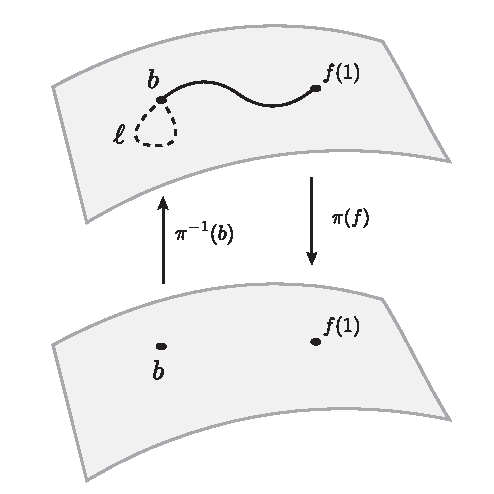
\includegraphics[width=0.4\textwidth]{fig/march/pathspace-fibration.pdf}
	\caption{Sketch of the path space fibration.}
	\label{fig:pathspace-fibration}
\end{figure}


\parhead{Check it's a fibration} This turns out to be a fibration in the following
sense. Take some space $ X $ and a homotopy into $ B $: $ h_t : X \to B $ (I am
using the Hatcher notation where one tucks the $ [0,1] $ portion of the homotopy
into a subscript).  Say we're also given a lift $ \tilde{h}_0 : X \to PB $,
which we choose to write as $ \tilde{h}_0(x) = (b, \gamma_x)\in PB $ for $ f : X
\to b \in B $, and $ \gamma_x : I \to B $ (here this 2-tuple notation denotes a
path $ \gamma_x $ starting at $ b $). 

The lift we construct is $ \tilde{h}_t = (B, \gamma_x \circ h_{[0,t]} (x))$,
where $ \circ $ here denotes path composition. Thus, this is a path starting at
$ b $, following $ \gamma_x $ (the lift of $ h $ the homotopy from $ X $ to $ B
$), then following $ h_s(x) $ along $ s \in [0,t] $, ending at $ h_t(x) $.
Notice $ t $ here is the parameterization coming from the homotopy $ h_t : X \to
B$, and the paramterization of $ \gamma_x \circ h_{[0,t]} (x)$ is that of $ PB
$:

\begin{center}
	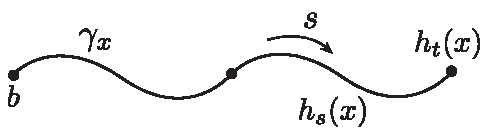
\includegraphics[width=0.5\textwidth]{fig/march/pathspace-hlp.pdf}
\end{center}

Thus, this is a path in $ PB $; then what is the projection $
\pi(\tilde{h}_t) $, i.e., its endpoint? Well, that's simply $ h_t(x) $. Thus $
\tilde{h}_t $ is indeed a lift and we can see the sense in which it is a
fibration.

What is the fiber $ \pi^{-1}(b) $? It is the space of loops based at $ b $. 
This is because $ \pi^{-1}(b) $ are precisely the paths which must end at $ b $
and start at $ b $. Thus we have a fibration $ \Omega B \to PB \to B $. 
See Hatcher, Prop. 4.64 for a generalization of this proof.
\entry{Third Homotopy of Compact Lie Group is Z}{3/9/24}
It is the case that for any simple, compact Lie group $ G $ one has $ \pi_3(G) 
= \mathbb{Z} $. Here I provide a sketch of a proof that this is the case. 

Apply the path fibration construction to $ G $:
\begin{equation*}
	\begin{tikzcd}
	X\times \left\{0\right\} \arrow[r, "\tilde{h}_0"] \arrow[d]
		& PG \arrow[d, "\pi"] \\
	X\times\left[0, 1\right] \arrow[r, "h"] \arrow[from=2-1, to=1-2, "\tilde{h}", dashrightarrow]
		& G
	\end{tikzcd}
\end{equation*}
with fiber $ \Omega G $ the loopspace. Every fibration grants us a long exact 
sequence of homotopy groups; in this case we have 
\begin{equation*}
	\cdots \to \pi_n(\Omega G) \to \pi_n(PG) \to \pi_n(G) \to \pi_{n-1}(\Omega G) 
	\to \pi_{n-1}(PG)\to \cdots 
\end{equation*}
But $ PG $ is contractible (they're just paths; while you might be worried that 
loops are not contractible, this is not the sense in which we are considering 
contraction. Here the appropriate way to think about it is as a line being
``sucked'' back into its starting point), so all homotopies 
vanish and in fact one has 
\begin{equation}\label{eq:pi3-z-les}
	\cdots \to \pi_n(\Omega G) \to 0 \to \pi_n(G) \to \pi_{n-1}(\Omega G) 
	\to 0 \to \cdots 
\end{equation}
Which implies that $ \pi_n(G) = \pi_{n-1}(\Omega G) $, and it suffices to compute 
$ \pi_{n-1}(\Omega G) $. This is an easier task because it is possible to 
approximate loops by geodesics, and geodesics of Lie groups are relatively
nice to work with. In particular, we may approximate a loop based at the origin 
$ e $ by $ k $ geodesics, all of which we take to be emanating from the origin 
of a copy of $ G $:
\begin{equation*}
	\Omega G \approx \text{geodesics of } S =\text{open subset of } G\times \overset{k}{\cdots}\times G
\end{equation*}
where one can take better and better approximations by cranking up $ k $. 
We are able to think of such a loop of broken geodesics as living in $ k $ 
copies of $ G $ because $ G $'s metric is biinvariant, a fact which is derived 
from its compactness.

Now one considers the energy functional $ E (\gamma) = (\int |\gamma|^2) $, for
which the geodesic is, by definition, a critical point (ideally, it minimizes
it, but this is a subtle matter). Conjugate points on this geodesics are points
such that any Jacobi field along $ \gamma $ keeps those points fixed (i.e., 
it vanishes at that point); alternatively, they are points such that there
exists a family of geodesics keeping those points fixed. The Morse index theorem
then tells us that the
number of such conjugate points is equal to the ``index'' of the Hessian of $
E(\gamma) $. 

Breaking this statement down: the Hessian is essentially a matrix of second
derivatives; it characterizes the critical point at which we are located.
Namely, the number of negative and positive eigenvalues characterizes the type
of critical point; e.g., for $ n_- $ negative eigenvalues and $ n_+ $ positive
eigenvalues one is at a saddle point with $ 2n_- $ ``decreasing directions''. $
n_- $ is the precisely the index of the Hessian. 

Thus we gain some geometric intuition for why the number 
of conjugate points of the geodesic is equal to the index: let's say we have a 
geodesic $ \gamma $ related by a Jacobi field to another geodesic $ \gamma' $
such that there are $ n $ conjugate points. The fact that $ \gamma' $ is also 
a geodesic means that we can't possibly be at a minimum of the energy functional, 
though we are at a critical point. This is only possible if there the energy 
functional decreases in certain directions in path space; there are as many 
such directions as there are sections of the geodesic pinned by conjuate points,  
as the conjugate points are necessarily shared as boundaries by a family of 
neighboring geodesics. 

\begin{center}
	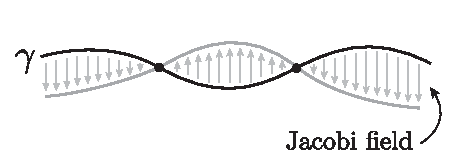
\includegraphics[width=0.5\textwidth]{fig/march/conjugate-points.pdf}
\end{center}

An additional two facts we need are (1) the index of geodesics of Lie groups is 
always even, and (2) the fundamental theorem of Morse theory: the space of paths 
from $ p $ to $ q $ is homotopic to a CW complex with one cell of dimension $
\lambda $ for each geodesic from $ p $ to $ q $ of index $ \lambda $. For (1),
one can compute this explicitly, but I don't find the computation particularly
insightful, so I am putting the matter aside until I can think of a more
intuitive way to see it (see
\href{https://mathoverflow.net/questions/66924/conjugate-points-in-lie-groups-with-left-invariant-metrics}{here}).
For (2), I hope it is relatively unsurprising upon some thought---it is a
special case of the fact that any manifold is a CW complex 
with a cell of dimension $ \lambda $ for each critical point of index $ \lambda $
(TODO understand this?).

So every geodesic has an even index, and the space of geodesics has an $ \lambda
$-cell for each geodesic of index $ \lambda $. Because we can approximate 
loops by geodesics, the space of loops only has even cells, and thus 
$ \pi_{1}(\Omega G) = 0$, and also, as a bonus, the cell complex has
\begin{equation*}
	\cdots\longrightarrow 0 \overset{\partial}{\longrightarrow} \mathbb{Z}\!\left\{2\text{-cells}\right\}
	\overset{\partial}{\longrightarrow} 0
\end{equation*}
(since there are no 1- or 3-cells), meaning that 
\begin{equation*}
	H_2(S) = \frac{\ker\partial =
	\mathbb{Z}\!\left\{2-\text{cells}\right\}}{\text{im}\,\partial = \left\{0\right\}}
	= \mathbb{Z}^t
\end{equation*}
for some $ t $ (the group is generated by $ t $ 2-cells). The Hurewicz theorem 
tells us for an $ n $-connected space the next higher ($ n+1 $) homotopy 
and homology groups agree; thus if $ G $ is path-connected, we have $ \pi_2(S) = 
H_2(S) =\mathbb{Z}^t $. But we've argued that $ S $ can be made to be a good 
enough approximation of $ \Omega G $; thus, we have $ \pi_2(\Omega G) =
\mathbb{Z}^t $ and $ \pi_3(G) = \mathbb{Z}^t $ since $ \pi_3(G) \simeq
\pi_2(\Omega G) $ by \cref{eq:pi3-z-les}. 

Now $ t $ here is related to the number of simple Lie groups that make $ G $ up. 
Thus, if $ G $ is simple we have $ t=1 $, which is what we want.

\subsection*{References}
\begin{itemize}[nosep]
\item Matt Noonan, Homotopy groups of Lie groups, URL (version: 2009-12-15):
	\url{https://mathoverflow.net/q/8957}
\item Milnor, Morse Theory (1960).
\end{itemize}

\entry{2+1 Electrodynamics}{...}

\entry{Dirac Quantization and Periodic Lagrange Multipliers}{3/15/24}
Consider a Dirac-quantization-like constraint on a field $ \phi $.
\begin{equation}\label{eq:periodic-dirac}
	\int_{\partial S} f[\phi] \in \mathbb{Z}
\end{equation}
Then consider some Lagrange multipler field $ \sigma(x) $ enforcing 
$ df[\phi] = 0 $. The path integral reads 
\begin{align}\label{eq:periodic-path-integral}
	\int \mathcal{D}\phi \mathcal{D}\sigma 
		\exp\left(i \int \mathcal{L}[\phi] + \sigma df[\phi] \right)
\end{align}
Consider what happens if we shift $ \sigma \to \sigma + 2\pi $:
\begin{align*}
	\int \mathcal{D}\phi \mathcal{D}\sigma 
		\exp\left(i \int \mathcal{L}[\phi] + \sigma df[\phi] + 2\pi df[\phi] \right)
\end{align*}
Now apply Stokes' theorem and \cref{eq:periodic-dirac} to the last term:
\begin{align*}
	&\int \mathcal{D}\phi \mathcal{D}\sigma 
		\exp\left(i \int \mathcal{L}[\phi] + \sigma d f[\phi] + i \int_{\partial S}2\pi f[\phi] \right)\\
		&\qquad
		= 
	\int \mathcal{D}\phi \mathcal{D}\sigma 
		\exp\left(i \int \mathcal{L}[\phi] + \sigma d f[\phi] + 2 \pi i N\right), \qquad N\in \Z
\end{align*}
But of course we can just extract $ \exp(2\pi i N) $ and set it to unity, so 
the path integral returns to the form \cref{eq:periodic-path-integral}.
Thus, as seen from the perspective of the path integral $ \sigma \sim \sigma + 
2\pi $.

any space z is whe to cell complex. whe $ \Longrightarrow $ h.e. by whitehead 

\entry{Instantons and Confinement}{...}

\entry{Continuum Limit of Gutzwiller Wavefunctions}{}

\entry{Bosonization in 2+1}{...}

\entry{Neural Quantum States}{3/16/24}
\begin{figure}[t]
	\centering
	\begin{subfigure}[b]{0.45\textwidth}
		\centering
		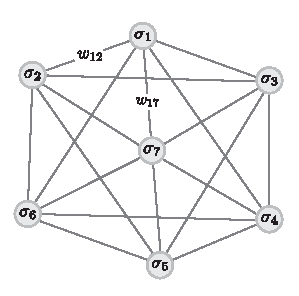
\includegraphics[width=\textwidth]{fig/march/boltzmann.pdf}
		\caption{Boltzmann machine.}
		\label{fig:boltzmann}
	\end{subfigure}
	\begin{subfigure}[b]{0.45\textwidth}
		\centering
		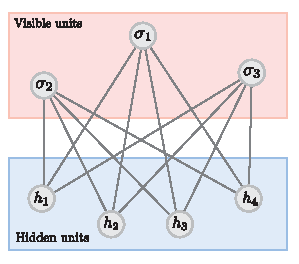
\includegraphics[width=\textwidth]{fig/march/restricted-boltzmann.pdf}
		\caption{Restricted Boltzmann machine. $ h_i $ do not connect to other 
		$ h_i $ and likewise for $ \sigma_i $.}
		\label{fig:restricted-boltzmann}
	\end{subfigure}
	\caption{}
\end{figure}
\subsection{(Restricted) Boltzmann Machines}
Boltzmann machines are a type of neural network which leverage insights from 
statistical physics to perform unsupervised learning of probabilistic models. 
That is, the goal is to use the Boltzmann machine to learn some target 
probability distribution $ P_{\text{T}}(X) $ given samples drawn from that 
probability distribution. 

The machine itself consists of a set of units $ \sigma_i $ and weights $ w_{ij} $
connecting each of those units (\cref{fig:boltzmann}). One defines an energy 
function 
\begin{equation}
	E(\sigma; w_{ij}, a_i) = \sum_i a_i \sigma_i + \sum_{ij} \sigma_i w_{ij} \sigma_j
\end{equation}
with biases $ a_i $ and weights $ w_{ij} $ connecting each unit to every other 
unit. The units themselves are binary with $ \pm 1 $ (some other authors choose $ 
\left\{0,1\right\} $). This model belongs to the class of \textbf{energy-based 
models}; such models leverage the fact that for an appropriately chosen 
$ E(v) $ (in the Boltzmann machine case, appropriately chosen $ w_{ij} $)
the target probability distribution---call this $ p_{\text{T}}(\sigma) $---can be
sufficiently approximated by the Boltzmann distribution
\begin{equation*}\label{eq:boltzmann-machine-distribution}
	p(\sigma) = \frac{1}{Z} e^{-E(\sigma; w_{ij}, a_i)}
\end{equation*}
where 
\begin{equation*}
	Z = \sum_{\left\{\sigma_i\right\}} \exp(-E (\sigma_i; w_{ij}, a_i))
\end{equation*}
is the partition function, i.e., the sum over all possible $ \sigma_i $ 
configurations that functions as a normalizing constant.

The model then trains $ w_{ij} $ by minizing some sort of measure of the 
divergence of $ p(\sigma) $ from $ p_{\text{T}}(\sigma) $---for instance 
maximum likelihood estimation or the Kullbach-Leibler divergence. Thus, given 
an unlabelled dataset $ \left\{\vbg{\upsigma}_n\right\} $ which is drawn 
from the unknown distribution $ p_{\text{T}} $, we may find $ E(\sigma; w_{ij},
a_i) $ such that $ p(\sigma) $ approximates $ p_{\text{T}} $. 

In practice, however, it is quite difficult to sample $ p(\sigma) $ for 
training purposes. The culprit is $ Z $, whose difficulty to evaluate is
well-known to physicists. One then resorts to the usual techniques employed 
to evaluate complex sums or integrals of this kind---chiefly, Monte Carlo
methods. We will see that the training of neural quantum states is no
different and we will need to employ Monte Carlo sampling of the wavefunction.

A special case of the Boltzmann machine that was designed with training
convenience in mind is the \textbf{restricted Boltzmann machine}. A restricted 
Boltzmann machine demotes a subset of $ \sigma_i $ to hidden units denoted $ h_i
$---these are units which do not appear as arguments to the probability
distribution $ p(\sigma_i) $ and whose purpose is analogous to a hidden layer 
in a feedforward network. Further, and crucially, we stipulate that the 
hidden units do not connect to themselves, only to visible units, and likewise 
for visible units (\cref{fig:restricted-boltzmann}). This amounts to writing $
\sigma_i w_{ij} \sigma_j$ as $ h_i w_{ij} \sigma_j $, so that 
\begin{equation*}
	E(\sigma_i; w_{ij}, a_i, b_i)
		= \sum_i a_i \sigma_i + \sum_i b_i h_i + \sum_{ij} h_i w_{ij} \sigma_j
\end{equation*}
(we have separated the bias into a visible bias $ a_i $ and a hidden bias 
$ b_i $).
The target probability distribution is approximated by the marginalization 
over $ h_i $---the trace, in physics parlance---so we must sum over $ h_i $
\begin{equation*}
	p(\sigma_i) 
		= \sum_{\left\{h_i\right\}} e^{-E(\sigma, h)}
\end{equation*}
The gradient (of the log) for the $ n $-th vector $ \vbg{\upsigma}_n $
\begin{align*}
	\frac{\partial \log p(\hat{\vbg{\upsigma}}_n)}{\partial w_{ij}}
		= \frac{1}{p(\hat{\vbg{\upsigma}}_n)} \frac{\partial p(\hat{\vbg{\upsigma}}_n)}{\partial w_{ij}}
		= \frac{1}{p(\hat{\vbg{\upsigma}}_n)} \left[
			\sum_{\left\{h_i\right\}} e^{-E(v,\hat{\vbg{\upsigma}}_n)} 
			\frac{\partial }{\partial w_{ij}} \left(\frac{1}{Z}\right) 
			+ \frac{1}{Z} \sum_{\left\{h_i\right\}} \frac{\partial }{\partial w_{ij}}
				e^{-E(h, \hat{\vbg{\upsigma}}_n)}
		\right]
		\\ 
		= \frac{1}{Z}\frac{1}{p(\hat{\vbg{\upsigma}}_n)} \left[
			-\sum_{\left\{h_i\right\}} e^{-E(v,\hat{\vbg{\upsigma}}_n)} \frac{1}{Z^2} \frac{\partial Z }{\partial w_{ij}} 
			- \frac{1}{Z} \sum_{\left\{h_i\right\}} 
			e^{-E(h, \hat{\vbg{\upsigma}}_n)} \hat{\sigma}_{n,i} h_j
			\right]
\end{align*}
The derivative of the partition function is 
\begin{align*}
	\frac{\partial Z}{\partial w_{ij}}
		= \frac{\partial }{\partial w_{ij}} 
			\sum_{\left\{h_i\right\}}
			\sum_{\left\{\sigma_i\right\}}
			e^{-E(h, \vbg{\upsigma}_n)}
		= \sum_{\left\{h_i\right\}}
			\sum_{\left\{\sigma_i\right\}}
			e^{-E(h, \vbg{\upsigma}_n)}
			(-\sigma_i, h_j)
		= - Z \langle \sigma_i v_j \rangle_{\text{model}}
\end{align*}
The subscript ``model'' says that this is the expectation value of the 
current forward pass Boltzmann machine distribution as opposed to the 
expectation value with respect to the data, which will show up shortly. 
Then we have 
\begin{align*}
	\frac{\partial \log p(\hat{\vbg{\upsigma}}_n)}{\partial w_{ij}}
		&= \frac{1}{p(\hat{\vbg{\upsigma}}_n)} \Bigg[
			\overbrace{\frac{1}{Z}\sum_{\left\{h_i\right\}} e^{-E(v,\hat{\vbg{\upsigma}}_n)}}^{p(\hat{\vbg{\upsigma}})}
			\frac{Z}{Z} \langle \sigma_i h_j \rangle_{\text{model}}
			- \overbrace{\frac{1}{Z} \sum_{\left\{h_i\right\}} 
			e^{-E(h, \hat{\vbg{\upsigma}}_n)}}^{p(\hat{\vbg{\upsigma}})}
			 \hat{\sigma}_{n,i} h_j
			\Bigg]\\
		&= \langle \sigma_i h_j \rangle_{\text{model}} 
			- \hat{\sigma}_{n,i} h_j
\end{align*}
Now, the gradient is the expected value over the training vectors $ \hat{\vbg{\upsigma}}_n $, 
so the derivative is
\begin{equation*}
	\frac{\partial \log p(\hat{\vbg{\upsigma}}_n)}{\partial w_{ij}}
	= \langle \sigma_i h_j \rangle_{\text{model}} 
		- \langle\hat{\sigma}_{n,i} h_j\rangle_{\text{data}}.
\end{equation*}
The benefit of the restricted Boltzmann machine is that there is an exact 
distribution that $ h_j $ follows given some $ \hat{\upsigma}_n $, so we 
can evaluate the second term. Let's say that $ h_k\in\left\{0,1\right\} $; 
the probability that $ h_k = 1$ given a visible unit can be calculated as follows. 
We have 
\begin{equation*}
	\frac{p(h_k=1\mid \sigma)}{p(h_k=0\mid \sigma)}
		= \frac{
			\exp\left[b_k + \sum_{i\neq k h_i b_i} + \sum_i v_i a_i + \sum_{i\neq k, j}h_i w_{ij} v_j
				+ \sum_j w_{kj} v_j\right]
		}{
			\exp\left[0\cdot b_k + \sum_{i\neq k h_i b_i} + \sum_i v_i a_i + \sum_{i\neq k, j}h_i w_{ij} v_j
				+ 0\cdot \sum_j w_{kj} v_j\right]
		}
\end{equation*}
Now, since $ h_k $ can only be in two states, $ p(h_k = 0\mid \sigma) = 1- p(h_k 0\mid\sigma)$, and 

\begin{align*}
	\frac{p(h_k=1\mid \sigma)}{1-p(h_k=1\mid \sigma)}
		&= \frac{
			\exp\left[b_k + \sum_{i\neq k h_i b_i} + \sum_i v_i a_i + \sum_{i\neq k, j}h_i w_{ij} v_j
				+ \sum_j w_{kj} v_j\right]
		}{
			\exp\left[\sum_{i\neq k h_i b_i} + \sum_i v_i a_i + \sum_{i\neq k, j}h_i w_{ij} v_j\right]
		}
		\\
		&=\exp\left(b_k + w_{kj} v_j\right)
\end{align*}
We can work out
\begin{equation*}
	p = e^W (1-p) \Longrightarrow (1+e^W) = e \Longrightarrow 
	p = \frac{e^W}{1 + e^W } \Longrightarrow \frac{1}{1+e^{-W}} = \sigma(-W)
\end{equation*}
So that the above implies
\begin{equation*}
	p(h_k = 1\mid \sigma) = \sigma(b_k + \sum_{j} w_{kj}v_j).
\end{equation*}
Notice that the argument relies on the fact that $ h_i $ does not connect 
to other hidden units. An identical argument finds 
\begin{equation*}
	p(\sigma_k = 1 \mid h) = \sigma(a_k + \sum_j w_{jk} )
\end{equation*}
Sampling $ \langle \sigma_i h_j\rangle_{\text{model}} $, however, remains
difficult. Strategies for doing so that leverage $ p(h_k=1\mid \sigma) $ and 
$ p(\sigma_k = 1\mid h) $ are described in Hinton. In the case of neural quantum 
states, however, the natural loss function is the energy of the system, and 
the gradients we must calculate are not the above. The evaluation will still 
be difficult, but in this case only because we must obtain the energy and its 
gradients indirectly in order to circumvent the curse of dimensionality. 

\subsection{Neural Quantum States}
One can view the many-body wavefunction $ \psi(\sigma_1, \dots, \sigma_N) $ 
appearing in 
\begin{equation*}
	\ket{\psi} = \sum_{\left\{\sigma_i\right\}} \psi(\sigma_1, \dots,\sigma_N)
		\ket{\sigma_1,\cdots, \sigma_N }
\end{equation*}
as a function from local degrees of freedom to a complex number, the amplitude, 
$ \psi : \left\{\sigma_i\right\} \to \C $. Thus we may treat $ \psi $ as a 
a Boltzmann machine with visible units $ \left\{\sigma_i\right\} $, albeit 
one that produces a complex number corresponding to the wavefunction as opposed 
to the probability amplitude. We thus provide $ \psi $ with a set of weights 
$ W = (w_{ij}, a_i, b_i)$ and hidden units $ h_i $ such that 
\begin{equation*}
	\psi(\sigma_1, \dots, \sigma_N; W)
		= \sum_{\left\{h_i\right\}}
			\exp\left(\sum_j a_j \sigma_j^z + \sum_i b_i h_i 
					+\sum_{ij} w_{ij} h_i \sigma_j^z \right)
\end{equation*}
Because $ \psi $ is complex-valued, $ w_{ij} $, $ a_i $, $ b_i $ are likewise 
taken to be complex valued. This is a restricted Boltzmann machine; we thus 
can explicitly marginalize $ \psi $:
\begin{align*}
	\psi 
		&= \sum_{\left\{ h_i \right\}}
			\exp\left(\sum_j a_j \sigma_j^z + \sum_i b_i h_i 
					+\sum_{ij} w_{ij} h_i \sigma_j^z \right)\\
	    &= \sum_{\left\{ h_i \right\}}
			\exp\left(\sum_j a_j \sigma_j^z\right) 
			\prod_i^M \exp\left(\sum_i b_i h_i\right) 
						\exp\left(\sum_j w_{ij} h_i \sigma_j^z\right)
\end{align*}
where we move the summation into the product as follows: 
\begin{align*}
	&= \exp \left( \sum_j a_j \sigma_j^z \right)
		\prod_i^M \sum_{h_i = \left\{ \pm 1 \right\}} 
			\exp\left(\sum_i b_i h_i\right)
			\exp\left(\sum_{ij} w_{ij} h_i \sigma_j^z\right) 
	\\ 
	&= \exp\left(\sum_j a_j \sigma_j^z \right)
	\prod_i^M \left[
		\exp\left(b_i + \sum_j w_{ij} \sigma_j^z \right)
		+ \exp\left(-b_i - \sum_j w_{ij} \sigma_j^z \right)
	\right]
	\\
	&= \exp\left(\sum_j a_j \sigma_j^z \right)
		\prod_i^M 2\cosh\left(b_i +\sum_{j} w_{ij} \sigma_j^z\right)
\end{align*}

\begin{thinnamedbox}[Note]
For some reason I always have to convince myself that the above move works, 
so for future reference here's the argument: we have a product indexed by 
$ i $ and a sum indexed by $ \ell $, which expanded looks like
\begin{align*}
	\prod_i^I \sum_\ell^L a_{i\ell}
		&= (a_{11} + a_{12} + \cdots + a_{1L})\\[-1em]
		&\qquad \times (a_{21} + \cdots + a_{2L})\\
		&\qquad \cdots \times (a_{I1} + \cdots + a_{IL})
\end{align*}
If we expand the products of sums, we obtain 
\begin{equation*}
	= a_{11} a_{21}\cdots a_{I1} + \cdots + a_{1L} a_{2L} \cdots a_{IL}
	= \sum_{a_{1i}}^L
	 \sum_{a_{2i}}^L \cdots
	 \sum_{a_{Li}}^L 
	 \prod_i^I a_{i\ell}.
\end{equation*}

\end{thinnamedbox}

Thus 
\begin{equation*}
	\psi(\sigma_1, \dots, \sigma_N; W)
	= 
	\exp\left(\sum_j a_j \sigma_j^z \right)
	\prod_i^M 2\cosh\left(b_i +\sum_{j} w_{ij} \sigma_j^z\right)
\end{equation*}

Given a Hamiltonian $ H $, how do we update $ w_{ij} $, $ a_i $, $ b_i $
to minimize the energy $ H = \bra{\psi}H\ket{\psi} $? As is typical with 
this type of problem, one resorts to a Monte Carlo method. Carleo and Troyer 
use a technique called stochastic reconfiguration wherein one updates the 
weights as 
\begin{equation*}
	W_{k+1, i}= W_{k,i} - \gamma_k S^{-1}_{k, ij} F_{k, j}
	\qquad (k=\text{iteration step})
\end{equation*}
where 
\begin{gather*}
	S_{k,ij} = \langle O_i^\dagger O_j\rangle - \langle O_i^\dagger\rangle \langle O_j\rangle,\qquad 
	F_{i} = \langle E_{\text{loc}} O_i^\dagger\rangle - \langle E_{\text{loc}}\rangle
		\langle O_i^\dagger \rangle\\
	O_i = \frac{1}{\psi} \partial_{W_i} \psi,\qquad 
	E_{\text{loc}} = \frac{1}{\psi}\bra{\left\{\sigma_i\right\}} H \ket{\psi} 
\end{gather*}
Here the expectation values denote $ \langle A\rangle = \sum_{\left\{\sigma_i\right\}} 
A (\left\{\sigma_i\right\})|\psi(\left\{\sigma_i\right\})|^2 $. They are 
evaluted with a Markov chain sampled with a Metropolis-Hastings procedure:
as is common with these VMC techniques, we flip a random spin and accept the 
new configuration with probability 
\begin{equation*}
	P(\left\{\sigma_i\right\}_k \to \left\{\sigma_i\right\}_{k+1})
		= \min \left(1, \Bigg| \frac{
				\psi(\left\{\sigma_i\right\}_{k+1})
			}{
				\psi(\left\{\sigma_i\right\}_{k})}\Bigg|^2\right).
\end{equation*}
Notice that we do not need to evaluate any Slater determinants and the
evaluation of the Metropolis-Hastings weight is fairly straightforward.
One caveat is that $ S $ is not guaranteed to be nonsingular; Carleo and Troyer 
circumvent this with an explicit regularization 
\begin{equation*}
	S_{ij}^{\text{reg}} = S_{ij} + \lambda_{k} \delta_{ij}S_{ij},\qquad 
	\lambda_{k} = \max (\lambda_0 b^k, \lambda_{\text{min}})
\end{equation*}
where their parameters are $ \lambda_{\text{min}} = 10^{-4}$, $ \lambda_0 = 100 $, 
$ b=0.9 $.

Stochastic reconfiguration is known in the machine learning literature as 
\href{https://agustinus.kristia.de/techblog/2018/03/14/natural-gradient/}{natural 
gradient descent}; there, what we call $ S $ is playing the role of the Fisher 
information matrix, and $ F $ plays the role of the gradient. In that sense it is a 
so-called ``preconditioning'' on the gradient as it takes the form of an 
adjustment to the gradient (the multiplication byt he inverse of the Fisher 
matrix).


\subsection*{References}
\begin{itemize}[itemsep=0.2ex]
\item Giuseppe Carleo, Matthias Troyer, \textit{Solving the quantum many-body problem
with artificial neural networks}. Science 355,602-606 (2017).
\href{https://doi.org/10.1126/science.aag2302}{DOI:10.1126/science.aag2302}. 
See the supplemental materials for information on their Monte Carlo sampling.
\item Torlai, Giacomo, and Roger G. Melko. \textit{"Learning thermodynamics with
Boltzmann machines."} Physical Review B 94.16 (2016): 165134.
\href{https://doi.org/10.1103/PhysRevB.94.165134}{DOI:10.1103/PhysRevB.94.165134}.
\item Grathwolh, et al., \textit{Your Classifier is Secretly an Energy Based Model and You Should Treat it Like One} (2019).
 \href{https://arxiv.org/abs/1912.03263}{arXiv:1912.03263}.
\item Hinton, \textit{A Practical Guide to Training
Restricted Boltzmann Machines}. \url{https://www.cs.toronto.edu/~hinton/absps/guideTR.pdf}.
\item Sorella, \textit{Green Function Monte Carlo with Stochastic Reconfiguration},
 \href{https://journals.aps.org/prl/abstract/10.1103/PhysRevLett.80.4558}{DOI:10.1103/ PhysRevLetter.80.5668}.
\end{itemize}


\entry{Poincar\'e Duality, Particle-Vortex, \& All That}{3/17/24}
\subsection{1 + 1}
\parhead{Bosonization}
\begin{equation}\label{eq:bosonization-fermion-integration}
	\int \mathcal{D} \psi \exp i  \left(
		\int d^2 x \left[
			-\bar{\psi}\slashed{\partial}\psi + i \bar{\psi} \slashed{A} \psi
		\right]	\right)
		= \exp \left(
			\frac{i}{4\pi}
			\int d^2 x F^{\mu\nu} \frac{1}{\partial^2} F_{\mu\nu}
		\right)
\end{equation}
The left-hand side is of course Gaussian, so we get the usual fermionic determinant: 
\begin{equation*}
	\int \mathcal{D}\psi \exp\left( \int d^2x -\bar{\psi} (i\slashed{\partial} 
		+ \slashed{A})\psi\right)
		= \det (i\slashed{\gamma} + \slashed{A})
\end{equation*}
How do we evaluate this determinant? There is an exercise in Jackiw, ``Topological 
Investigations of Quantized Gauge Theories'' which provides a 1d sketch of 
how to do so. The story is like this: One thinks of this determinant as 
the effective energy 
\begin{equation*}
	W[A] = -i \ln \det( \slashed{\partial} - \slashed{A}), \qquad 
	e^{iW[A]} = \langle 0\vert 0 \rangle _A
\end{equation*}
(that is, we are viewing the path integral as the vacuum-vacuum correlation function)
so that we may substitute the Green's function for $ \slashed{\partial} $: 
\begin{equation*}
	(\slashed{\partial} - i\slashed{A}) G = \delta(x) - iG\slashed{A}
\end{equation*}
Using $ \det M = \exp \ln M $ we write 
\begin{equation*}
	\ln \det(\slashed{\partial} - i\slashed{A}) 
		= \ln \exp(\tr \ln (\delta - iG\slashed{A}))
		= \tr \ln(\delta - iG \slashed{A})
\end{equation*}
One expands the log and finds that only the first order term contributes.
{\color{myred}(I wasn't sure how this was the case.  Perhaps it had something to
do with the step functions.)} Then we substitue $ G $ for $ i\langle\text{propagator}\rangle $
and find
\begin{equation*}
	-i\tr G e\slashed{A} = \int dt A(t)
\end{equation*}
In $ 1+1 $d one supposedly finds 
\begin{equation*}
	\int dx dy A^\mu(x) G_{\mu\nu}A^\nu(y)
\end{equation*}
with $ G_{\mu\nu} = [g_{\mu\nu} - \partial_\mu\partial_\nu/\partial^2]\delta(x-y)$
for the vector current propagator. This is a classic result owing to the famed 
Schwinger paper in which he introduces what we now call the Schwinger model. 
At any rate I could not really piece together the story for $ 1+1 $, and 
even taking for granted the above equation I could not get the form in 
\cref{eq:bosonization-fermion-integration}. One thought was to leverage 
$ \partial^2 = g^{\mu\nu}\partial_\mu \partial_\nu \Longrightarrow 
g_{\mu\nu} = \partial_\mu\partial_\nu/\partial^2 $ but I was still far from 
the desired result.


\parhead{T-duality}


\subsection{2 + 1}
\parhead{Particle-vortex} Consider the abelian Higgs model:
\begin{equation*}
	S = \int d^3 x \left[
		- \frac{1}{2} |\mathcal{D}_\mu \phi|^2
			- V(|\phi|) - \frac{1}{4} F_{\mu\nu}^2
	\right]
\end{equation*}
The field $ \phi $ admits vortex configurations $ \phi = \phi_0(r)
\exp(i\alpha(\theta)) $ where $ \alpha(\theta) = N\theta $ and $ N $ is the
winding number of the vortex. 
We split the field configuration into vortex solutions and smooth solutions 
$ \phi = \phi_0 \exp(i\alpha_{\text{V}} + i \alpha_{\text{S}}) $, so that 
the kinetic term becomes 
\begin{align*}
	|\mathcal{D}_\mu \phi|^2
		&= |\partial_\mu \phi_0 \cdot e^{i\alpha} 
			+ \phi_0 \partial_\mu e^{i\alpha_{\text{V}} + i\alpha_{\text{S}}}
			+ ie a_\mu \phi_0 e^{i\alpha}|^2\\
		&= |\partial_\mu \phi_0\cdot e^{i\alpha}
		 	+ i\phi_0 e^{i\alpha}(\partial_\mu \alpha_{\text{V}} 
			+ \partial_\mu \alpha_{\text{S}}) + iea_\mu \phi_0 e^{i\alpha}|^2\\
		&= |\partial_\mu \phi_0 \cdot e^{i\alpha}
		 	+ i\phi_0 e^{i\alpha}(\partial_\mu \alpha_{\text{V}} 
			+ \partial_\mu \alpha_{\text{S}} + ea_\mu)|^2\\
		&= \underbrace{|e^{i\alpha}|^2}_{=1}
		  |\partial_\mu \phi_0
		 	+ i\phi_0 (\partial_\mu \alpha_{\text{V}} 
			+ \partial_\mu \alpha_{\text{S}} + ea_\mu)|^2
\end{align*}
All the quantities involved in the second factor are real so this is just 
the square modulus of a complex number: 
\begin{equation*}
	\mathcal{D}_\mu \phi 
		= |\partial_\mu\phi_0|^2 + \phi_0^2 
			\left(\partial_\mu \alpha_{\text{V}} + \partial_\mu \alpha_{\text{S}}\right)^2
\end{equation*}
Note that because the curl of a gradient vanishes, we have $ \epsilon^{ij}\partial_i 
\partial_j \alpha = 0 $ everywhere except at the vortices. We use the shorthand 
$ b_\mu = \partial_\mu \alpha $ and enforce the aforementioned constraint
(now reading $ \epsilon^{\mu\nu\rho} \partial_\mu b_\nu = 0$) via a Lagrange
multiplier field $ \lambda_\mu $. The action now reads 
\begin{equation}\label{eq:abelian-higgs-action}
	S  = \int d^3 x \left[
		- \frac{1}{2} |\partial_\mu \phi_0|^2 
		- \frac{1}{2} \phi_0^2 \left(
			b_{\mu, \text{S}} + b_{\mu, \text{V}}
				+ ea_\mu
		\right)^2 
		+ \lambda_\mu \epsilon^{\mu\nu\rho} \partial_\nu b_{\rho, \text{S}}
		+ \cdots
	\right]
\end{equation}
The equation of motion of $ b_{\mu,\text{S}} $ is 
\begin{equation}\label{eq:abelian-higgs-eom}
	\frac{\partial \mathcal{L}}{\partial b_{\mu, \text{S}}}
	- \partial_\nu \frac{\partial \mathcal{L}}{\partial_\nu b_{\mu,\text{S}}}
		= 0 
\end{equation}
There's some index rearranging to peform to obtain the second term: the derivative 
appears in $ \lambda_\mu \epsilon^{\mu\nu\rho} \partial_\nu b_{\rho, \text{S}}$
which we can rewrite as $ \lambda_\rho \epsilon^{\rho \nu \mu} \partial_\nu
b_{\mu,\text{S}} = - \lambda_\rho \epsilon^{\mu \nu \rho} \partial_\nu
b_{\mu,\text{S}} $ by relabelling indices and rearranging the
antisymmetric tensor. We then have 
\begin{equation*}
	\partial_\nu \frac{\partial \mathcal{L}}{\partial_\nu b_{\mu,\text{S}}}
	= \partial_\nu  \frac{\partial}{\partial_\nu b_{\mu,\text{S}}} 
		\left(\lambda_\rho \epsilon^{\mu \nu \rho} \partial_\nu
		b_{\mu,\text{S}} \right)
	= \partial_\nu \lambda_\rho \epsilon^{\mu\nu\rho}
\end{equation*}
Meanwhile, 
\begin{equation*}
	\phi_0^2 \left(
		b_{\mu, \text{S}} + b_{\mu, \text{V}}
			+ ea_\mu
	\right)^2 
		= \phi_0^2 \left(
			b_{\mu,_{\text{V}}}^2 
			+ b_{\mu,_{\text{S}}}^2 
			+ e^2 a^2_\mu 
			+ 2 b_{\mu,_{\text{V}}} b_{\mu,_{\text{S}}}
			+ 2 b_{\mu,\text{V}} ea_\mu
			+ 2 b_{\mu,\text{S}} ea_\mu
		\right)
\end{equation*}
so 
\begin{equation*}
	\frac{\partial \mathcal{L}}{\partial b_{\mu, \text{S}}}
		= -\phi_0^2 (b_{\mu,\text{S}} + b_{\mu,\text{V}} + ea_\mu )
\end{equation*}
and \cref{eq:abelian-higgs-eom} is 
\begin{equation*}
	\phi_0^2 (b_\mu + ea_\mu) = \epsilon^{\mu\nu\rho}\partial_\nu \lambda_\rho
	\iff 
	b_\mu = \frac{\epsilon^{\mu\nu\rho} \partial_\nu \lambda_\rho}{\phi_0^2}
		-e a_\mu
\end{equation*}
Now we substitute this into \cref{eq:abelian-higgs-action} to eliminate
$ b_{\mu,\text{S}} $ and find the dual action. First we find 
\begin{equation*}
	\phi_0^2 \left(
			b_{\mu, \text{S}} + b_{\mu, \text{V}}
				+ ea_\mu
		\right)^2 
		= \frac{1}{\phi_0^2} (\epsilon^{\mu\nu\rho} \partial_\nu \lambda_\rho)^2
		= \frac{1}{2\phi_0^2}(\partial_\mu \lambda_\nu - \partial_\nu \lambda_\mu)^2.
\end{equation*}
Using 
\begin{equation*}
	b_{\mu, \text{S}} = 
		\frac{\epsilon^{\mu\nu\rho} \partial_\nu \lambda_\rho}{\phi_0^2}
			- b_{\mu, \text{V}} - e a_\mu
\end{equation*}
we can substitute into the Lagrange multiplier term to find
\begin{equation*}
	\epsilon^{\mu\nu\rho}\lambda_\mu \partial_\nu b_{\rho, \text{S}}
	= \frac{1}{\phi_0^2} \lambda_\mu \epsilon^{\mu\nu\rho} \epsilon^{\rho\lambda\sigma}
		\partial_\nu \partial_\lambda \lambda_\sigma
		- \epsilon^{\mu\nu\rho} \lambda_{\mu}\partial_\nu b_{\sigma, \text{V}}
			- e \epsilon^{\mu\nu\rho} \lambda_\mu\partial_\nu a_\mu
\end{equation*}
where supposedly the first term vanishes. We recognize the second term as the
vortex current 
\begin{equation*}
	j_\text{vortex}^\mu 
		= \frac{e}{2\pi} \epsilon^{\mu\nu\rho} \partial_\nu b_{\rho}
		= \frac{1}{2\pi \phi_0^2} \epsilon^{\mu\nu\rho} \partial_\nu j_\rho
\end{equation*}
where $ j_\rho $ is the $ \text{U}(1) $ Noether current. This current is 
conserved by virtue of the (topological) fact that the curl of a divergence 
should vanish; thus it is an example of a topological current, one whose 
conservation is ensured by topology of the field configuration. One might think
it funny to view it as a current, seeing as as which symmetry it is associated 
with is unclear. It is arguably this very question---what symmetry this current 
is associated with---that motivates the introduction of generalized symmetries.
For instance, if we consider $ \text{U}(1) $ theory, invariance under a 1-form 
symmetry characterizes a lack of vortices (which are charged under this symmetry).
In fact, it is often the case that the generalized symmetry in the original 
theory is understood as a conventional symmetry in the dual theory. 

At any rate, the dual action is 
\begin{equation*}
	S = \int d^3 x 
		\left[
			- \frac{1}{4\phi_0^2}(\partial_\mu \lambda_\nu - \partial_\nu \lambda_\mu)^2 
			- \frac{1}{2} \epsilon^{\mu\nu\rho} \lambda_\mu \partial_\nu b_{\rho,\text{V}}
			- e\epsilon^{\mu\nu\rho}\lambda_\mu \partial_\nu a_\mu
			+ V(\phi_0) + F_{\mu\nu}^2
		\right].
\end{equation*}
Now note that in \cref{eq:abelian-higgs-action} $ \phi_0^2 $ plays the role of the kinetic 
coupling for $ (\mathcal{D}_\mu \alpha)^2 $ whereas in the dual action the 
$ b $ field has $ 1/\phi_0^2 $; thus this is indeed a weak/strong duality.

\subsection{Poincar\'e Duality}
Current is some charge distirbution dirac delta, then hodge dual to other 
current

d - n topological current (some defect in an otherwise smooth function) is dual 
to original n funciton.


\subsection*{References} 
\begin{itemize}[itemsep=0.2ex]
\item Jackiw, ``Topological Investigations of Quantized Gauge Theories,''
	\textit{Current Algebra and Anomaly}.
\item N\u astase, \textit{String Theory Methods for Condensed Matter Physics}, Ch. 21. 
	Note N\u astase uses $ b_\mu $ for the Lagrange multipliers and $ \lambda_\mu $
	for $ \partial_\mu \alpha $. Lagrange multipliers are usually denoted $ \lambda $
	so I switched his notation.
\end{itemize}


\entry{Fast Computation of VMC Determinants}{3/18/24}
In a Monte Carlo simulation of a strongly correlated system one needs the 
ratio 
\begin{equation*}
	\frac{\braket{x'\vert\Phi}}{\braket{x\vert\Phi}}
\end{equation*}
where $ x' $ is a proposed classical configuration and $ x $ is the present 
configuration. Of course, given a set of single-particle wavefunctions, the 
many-body wavefunction $ \braket{x\vert \Phi} $ is some Slater determinant 
of the form 
\begin{equation*}
	\det U = 
	\begin{bmatrix}
		\phi_1(x_1) & \phi_2(x_1) & \cdots & \phi_N(x_1)\\ 
		\phi_1(x_2) & \phi_2(x_2) &        & \phi_N(x_2)\\ 
		\vdots      &             & \ddots &            \\ 
		\phi_1(x_N) & \phi_2(x_N) &        & \phi_N(x_N)
	\end{bmatrix}
\end{equation*}
(we ignore the spin d.o.f.; reintroducing it simply amounts to a product of 
Slater determinants for up and down spins). We have made the arbitrary choice 
to index the wavefunction along the columns and the particle along the rows; 
of course the other option is obtained by a transpose. Now, calculating this 
determinant is at best an $ O(N^3) $ task---assuming that the number of particles 
is an extensive quantity we will quickly run into unfeasibly long simulation 
times for more than a few decimal places' accuracy on a larger than $ 4\times 4 $
lattice. 

The cleverer way to go about this is to tabulate from the get-go all possible
weights that we might encounter. Fortunately, this is not a difficult thing 
to calculate; the first thing we need is a matrix of the same form as above, 
only with a row with every possible site: 
\begin{equation*}
	\det \tilde{U} = 
	\begin{bmatrix}
		\phi_1(r_1) & \phi_2(r_1) & \cdots & \phi_N(r_1)\\ 
		\phi_1(r_2) & \phi_2(r_2) &        & \phi_N(r_2)\\ 
		\vdots      &             & \ddots &            \\ 
		\phi_1(r_L) & \phi_2(r_N) &        & \phi_N(r_N)
	\end{bmatrix}
\end{equation*}
Observe that one can recover the slater matrix $ U $ by selecting those 
rows of $ \tilde{U} $ that correspond to occupied sites.
As it turns out, the following matrix will contain the weights 
\begin{equation}\label{eq:vmc-weight}
	W = \tilde{U} U^{-1},\qquad 
	W_{K,\ell} = \frac{\det U'}{\det U}
		= \frac{\braket{x'\vert \Phi}}{\braket{x \vert \Phi}}
\end{equation}
where $ x' $ differs from $ x $ by the particle $ x_\ell $ hopping to the site 
$ r_K $. Here $ U $ is $ N \times N$ matrix, $ \tilde{U} $ is $ L\times N $
($ L $ is the total number of sites), and thus $ W $ is $ L\times N$.
Of course, upon accepting $ x' $, $ W $ changes by virtue of the appearance of 
$ U $, which depends on the configuration. Then the matrix $ W $ can be updated 
as 
\begin{equation*}
	W_{I,j}' 
		= W_{I,j} - \frac{W_{I,\ell}}{W_{K,\ell}} (W_{K,j} - \delta_{\ell,j}),
		\qquad ( x_\ell \to r_K )
\end{equation*}
Here $ \delta_{\ell, j}$ is essentially the zero matrix with the $ \ell $-th 
column filled with ones. If only one particle is moved, this can be written 
as a rank-1 (dyadic) update 
\begin{equation*}
	W'_{I,j} = W_{I,j} + a_I b_j,\qquad 
	a_I = W_{I,\ell},\quad b_j = - \frac{1}{W_{K,\ell}}(W_{K,j}- \delta_{\ell, j})
\end{equation*}
For implementation it is easier to think of this as the outer product
\begin{equation*}
	W' = W + \mathbf{a} \mathbf{b}^T
\end{equation*}
where it is crucial that we take the transpose and not the complex conjugate. 
Of course round-off errors might accumulate and at long simulation times this 
updating is susceptible to numerical instability. It is thus customary to 
occasionally recalculate $ W $ directly from the Slater matrix with
\cref{eq:vmc-weight}; at 64-bit precision this recalculation takes place on 
the order of a few million timesteps. Roundoff errors might also lead to large 
fluctiations on account of the matrix inverse of \cref{eq:vmc-weight}---an error 
of order $ \epsilon $ of course becomes $ 1/\epsilon $ and one observes
disproportionally large weights which do not affect the acceptance
probability (at that timestep) but contaminate other matrix entries. In such 
situations it is necessary to round off elements of $ W $ at, say, roughly 
15 decimal points for 64-bit precision floats.

\subsection*{References} 
\begin{itemize}[itemsep=0.2ex]
\item Becca, Sorella, \textit{Quantum Monte Carlo Methods for Strongly Correlated 
	Systems} (2017).
\end{itemize}

\entry{Local Unitary Transformations and Phase Transitions}{3/26/24}
Does symmetry local unitary transformation still connect two states in same 
phase iff there's no gap closing?

% Consider a 

\subsection*{References}
\begin{itemize}[itemsep=0.2ex]
	\item Chen, Gu, Wen, \textit{Local unitary transformation, long-range quantum
	entanglement, wave function renormalization, and topological order}.
	\url{https://arxiv.org/abs/1004.3835}.
\end{itemize}

\entry{Stationary Phase and Time Evolution in QM}{3/27/24}


\entry{SPTs}{...}
\subsection{MPS Refresher}
Matrix product states (MPS) take the form
\begin{equation}\label{eq:mps}
	\ket{\psi} = \sum_{\left\{ j_i \right\}}
		A^{(j_1)}_{\hphantom{(j_1)}\mu_1}
		A^{(j_1)\mu_1}_{\hphantom{(j_1)}\mu_2}
		A^{(j_1)\mu_3}_{\hphantom{(j_1)}\mu_3}
		\cdots
		A^{(j_{n-1})\mu_{n-1}}_{\hphantom{(j_1)}\mu_{n-1}}
		A^{(j_n)\mu_{n}} \ket{j_1 \cdots j_n}
\end{equation}
where $ A^{(j_i)\mu_i}_{\hphantom{(j_i)} \mu_i}$ are $ \chi\times \chi $
matrices for bond size $ \chi $ (viewed as rank-3 tensors if we include the 
additional index $ j_i $). They are ansatze wavefunctinos which leverage the
local nature of entanglement to model to great approximation ground states of 
gapped systems. DMRG is for instance nothing more than a variational technique
that explores the space of MPSs.

How do MPS leverage local entanglement struture? Consider some general state 
\begin{equation*}
	\ket{\psi} 
		= \sum_{\left\{j_i\right\}} \psi(j_1, \dots, j_n)\ket{j_1, \dots,j_n}
\end{equation*}
here $ \ket{j_i} $ is a basis labelling the site degree of freedom; ultimately 
we want to express the wavefunction in this basis. Now, we are guaranteed 
a Schmidt decomposition of any state:
\begin{equation*}
	\ket{\psi}
	= \sum_{\alpha} \Lambda^{(\alpha)} \ket{\alpha_{\text{L}}}\ket{\alpha_{\text{R}}}
\end{equation*}
The strategy is to proceed along the chain and successively perform Schmidt 
decompositions at each site. We will see that this affords us a physically 
justifiable (and thus, one hopes, sufficiently accurate) reduction in the number of
parameters we need to express the wavefunction.

To illustrate, the first two sites will proceed as 
\begin{equation*}
	\ket{\psi} = \sum_{\alpha^1} A^{(\alpha^1)} \ket{\alpha^1_1} \ket{\alpha^1_{2\cdots n}}
		= \sum_{\alpha^1, \alpha^2} A^{(\alpha^1)}A^{(\alpha^2)}
		\ket{\alpha^1_1}\ket{\alpha^1_2}\ket{\alpha^2_{3\dots n}}
\end{equation*}
here $ A^{(\alpha^i)} $ are the Schmidt coefficients for that particular site, 
and $ \alpha^i_{1\dots m-1},\alpha^i_{m\dots n} $ label the states in our Schmidt basis for the 
decomposition partitoning the sites $ m,\dots,n $.
We can treat $ A^{(\alpha_i)}=  A^{(\alpha_i)\mu_i}_{\hphantom{(\alpha_i)} \mu_i+1} $ 
diagonal matrix without loss of generality, for reasons that will become clear shortly.
The dimension of this matrix is the size of the Schmidt basis, i.e., there is a 
diagonal entry for each $ \alpha_i $. 
The number of labels $ \alpha^1 $ will depend on the particular site in the
chain; as we move along, the number of labels will grow (as the number of states
needed to form a basis exponentially with the number of sites).
The key approximation that MPSs make is to keep only the $ \chi $ lowest 
Schmidt values---the idea is that entanglement should remain relatively localized 
...

Thus one obtains a decomposition 
\begin{equation*}
	\sum_{\left\{\alpha_i\right\}} 
		\Lambda^{(\alpha_1) }_{\hphantom{(\alpha_1)} \mu_1}
		\Lambda^{(\alpha_2) \mu_1}_{\hphantom{(\alpha_1)} \mu_2}
		\cdots 
		\Lambda^{(\alpha_{n-1}) \mu_{n-2}}_{\hphantom{(\alpha_{n-1})} \mu_{n-1}}
		\Lambda^{(\alpha_n) \mu_{n-1}}_{\hphantom{(\alpha)} }
		\ket{\alpha_1 \dots\alpha_n}
\end{equation*}
At this point we only need to express this in site basis $ j_i $ by means 
of a change of basis matrix $ \Gamma^{(j_i) \nu_{i}}_{\hphantom{(j_i)} \mu_i} 
= \langle j_{i, \mu} \vert \alpha_{i,\nu} \rangle$: 
\begin{equation*}
	\sum_{\left\{ j_i \right\}}
		\Lambda^{(j_1)}_{\nu_1} \Gamma^{(j_1)\nu_1}_{\hphantom{(j_1)} \mu_2}
		\Lambda^{(j_2)\mu_2}_{\hphantom{(j_2)}\nu_2} \Gamma^{(j_2)\nu_2}_{\hphantom{(j_i)} \mu_3}
		\cdots 
		\Lambda^{(j_n)\mu_n}_{\hphantom{(j_n)}\nu_n} \Gamma^{(j_n)\nu_n}_{\hphantom{(j_i)} }
		\ket{j_1\dots j_n}
\end{equation*}
If we call $ \Lambda^{(j_n) \mu_i}_{\hphantom{(j_n)}\nu_i}\Gamma^{(j_i) 
\nu_{i}}_{\hphantom{(j_i)} \mu_{i+1}} = A^{(j_i)\mu_i}_{\hphantom{(j_i)} \mu_{i+1}}$ 
we recover the form of \cref{eq:mps}. 
	

\entry{Useful Field Theory Formuale}{3/27/24}
\begin{equation*}
	T^{\mu\nu} = \frac{\delta \mathcal{L}}{\delta \partial_\mu \phi}
		\partial^\nu \phi - g^{\mu\nu}\mathcal{L}
\end{equation*}
\begin{equation*}
	\mathcal{H}
		= \frac{\delta \mathcal{L}}{\delta \partial_0 \phi}	
			\partial^0 \phi
			- g^{00} \mathcal{L}
\end{equation*}

\entry{Avoided Crossings and Symmetry}{3/28/24}
There is lore in the many-body literature that eigenvalues of a system 
undergoing an adiabatic evolution only cross if the eigenstates have different 
symmetries. Here's more or less how this works. Consider a diagonalized 
Hamiltonian $ H $ perturbed by a term $ H' $
\begin{equation*}
H + H' = 
	\begin{bmatrix}
		E_1 & 0 \\ 0 & E_2 
	\end{bmatrix}
	+ \begin{bmatrix}
	0 & \Delta \\ \Delta^\ast & 0 
	\end{bmatrix}
	= \begin{bmatrix}
	E_1 & \Delta \\ \Delta^\ast & E_2
	\end{bmatrix}
\end{equation*}
(without loss of generality we take the perturbation to be completely off-diagonal). 
The spectrum of this Hamiltonian consists of 
\begin{gather*}
	\ket{\psi_{\pm}} = \phi_{\pm}\ket{E_1} - \ket{E_2},\qquad 
	E_\pm = E_1 + E_2 \pm \sqrt{(E_1 - E_2)^2 + 4 |\Delta|^2}\\ 
	\phi_{\pm} 
		= E_1 - E_2 \pm \sqrt{(E_1 - E_2)^2 + 4|\Delta|^2}
\end{gather*}
Observe $ E_{\pm} $: since $ |\Delta|^2 $ is nonnegative, we can only have 
$ E_+ = E_- $ if $ E_1 = E_2 $ and $ \Delta = 0 $. This is an avoided crossing; 
we think of $ \Delta $ as depending on some adiabatically varied parameter 
such that if any two eigenvalues are well represented by an effective $ 2\times
2 $ Hamiltonian as above, the energy levels cannot cross for any value of $
\Delta $.

This argument relies, however, on the mixing between $ \ket{E_1} $ and $
\ket{E_2} $. Superselection rules prevent, however, (adiabatic) evolution from a
state in one irrep to another; more precisely we cannot adiabatically evolve 
into a superposition of states with two different symmetries. Thus, in our 
effective two-level system, $ \ket{E_1} $ and $ \ket{E_2} $ must enjoy the 
same symmetry; if they do not, they cannot mix and the energy levels can cross. 
(Is this in contradiction with the relationship beween degeneracy and symmetry? 
Not if you can have degeneracies that don't descent from symmetries.)


%%%%%%%%%%%%%%%%%%%%%%%%%%%%%%%%%%%%%%%%%%%%%%%%%%%%%%%%%%%%%%%%%%%%%%%%%%%%%%%%
%%%%%%%%%%%%%%%%%%%%%%%%%%%%%%%%%%%%%%%%%%%%%%%%%%%%%%%%%%%%%%%%%%%%%%%%%%%%%%%%

\chapter{April}
\begin{tocbox}
	\minitoc
\end{tocbox}

\entry{Is RG a semigroup?}{4/1/24}

\entry{}{}
Integer quantum hall effect - we have a harmonic oscillator portion of the 
solution (in direction of applied magnetic field?), the quantization of which 
is the Landau level $ \nu $. Notice that if the landau level is completely filled, 
we have a gap. The edge modes carry the current; there are $ \nu $ different 
``channels'' for the modes. One can use Landauer electron transport theory to 
find that for each such channel we have $ e^2 V_H/h $ current.

\entry{EFT of the Hubbard Model}{4/6/24}
Consider the Hubbard Hamiltonian ($ a $ indexes spin)
\begin{equation*}
	H = -t \sum_{j = 1}^{L} (c_{j,a}^\dagger c_{j+1, a} + c_{j+1, a}^\dagger 
							c_{j,a})
			+ \sum_{j = 1}^{L} u(1-2n_{j\uparrow})(1-2n_{j\downarrow})
\end{equation*}
One can consider the continuum limit of the Hubbard model---first write 
$ \ell = L a_0 $, i.e., split the chain into $ L $ segments of lattice spacing 
$ a_0 $. In this case the position $ x $ is $ na_0 $. The continuum field
operator in terms of the real and wavenumber space operators is
\begin{equation*}
	\psi_a(x) = \lim_{a \rightarrow \infty}
		\frac{c_{n,a}^\dagger}{\sqrt{a_0}}
		= \frac{1}{\sqrt{\ell}}\sum_{k=-\infty}^\infty
			e^{-iq_k x}c_{k,a}^\dagger 
\end{equation*}
where $ c_k = 2\pi k/\ell $. The inverse is then 
\begin{equation*}
	c_{k,a}^\dagger = \frac{1}{\sqrt{\ell}}
		= \int_0^\ell dx e^{iq_k x} \psi_a^\dagger (x) 
\end{equation*}
Bearing in mind that the continuum limit takes the sum to an integral as 
\begin{equation*}
	\sum_{j=1}^L a_0 f(na_0)
		\xrightarrow{a_0 \to \infty}
		\int_0^1 dx f(x)
\end{equation*}
(of course we could shift $ (0, \ell) \to (-\ell/2, \ell/2) $ and $ \ell\to
\infty $ for the infinite system limit). The kinetic term becomes 
\begin{align*}
	-t \sum_{j=1}^L \left(
		c_{j,a}^\dagger c_{j+1, a} + c_{j+1, a}^\dagger c_{j,a}
	\right)
	= -t \sum_j a_0 
		\left( \frac{1}{a_0} c_{j,a}^\dagger c_{j+1, a} 
			+ \frac{1}{a_0} c_{j+1, a}^\dagger c_{j,a}\right)\\ 
	= - t \int dx (\psi_a^\dagger \psi_a(x + a_0) + \psi_a(x+a_0)^\dagger \psi_a(x))
\end{align*}
Now, recall that translations are generated by
\begin{equation*}
	\psi(x + a_0) = e^{a_0 \partial_x} \psi(x) 
		= \psi(x) + a_0 \partial_x \psi(x) + \frac{1}{2}a_0^2 \partial^2_x \psi(x) 
			+ \cdots 
\end{equation*}
Consequently, we can write 
\begin{align*}
	&\psi_a(x)^\dagger \psi_a(x + a_0) + \psi_a(x+a_0)^\dagger \psi_a(x)\\
	&\qquad= \psi_a ^\dagger \left(\psi_a + a_0\partial_x \psi_a 
		+ \frac{1}{2}a_0^2 \partial_x^2 \psi_a\right)
		+ \left(\psi_a^\dagger + a_0 \partial_x \psi_a^\dagger 
		+ \frac{1}{2}a_0^2 \partial_x^2 \psi^\dagger \right) \psi_a\\
	&\qquad= 2 \psi_a^\dagger \psi_a + a_0 \left(
		\psi_a^\dagger \partial_x \psi_a + \partial_x \psi_a^\dagger \psi_a
	\right)
		+ \frac{a_0^2}{2}\left(
			\psi_a^\dagger \partial_x^2 \psi_a + \partial_x^2 \partial_a^\dagger \psi_a
		\right)\\
	&\qquad =2  \psi_a^\dagger \psi_a + a_0 \partial_x(\psi_a^\dagger \psi_a)
		+ \frac{a_0^2}{2}\left(
			\partial_x^2(\psi_a^\dagger \psi_a) - 2(\partial_x \psi_a^\dagger)
			(\partial_x \psi_a)
		\right)
\end{align*}
If we assume the fields aren't supported at the boundaries, the total derivative 
terms vanish, and we're left with 
\begin{equation*}
	\int dx \left[
		-2t \psi_a^\dagger \psi_a + ta_0^2 (\partial_x \psi_a)^2
	\right]
\end{equation*} 
Now, the first term is an IR divergence which ultimately may be ignored.  The
interaction term is 
\begin{align*}
	a_0u(1-2n_{j\uparrow})(1-2n_{j\downarrow})
		= a_0\pm u(1+2n_{j\uparrow} - 2n_{j\downarrow} + 4n_{j\uparrow} n_{j\downarrow})\\
		= \pm u \left(a_0 - 2 \psi_a^\dagger \psi_a 
			+ \frac{2}{a_0} \psi_a^\dagger \psi_b^\dagger \psi_a \psi_b \right)
\end{align*}
The sign ambiguity comes from different continuum limits corresponding to the 
Shiba transformation of the $ c_{j,a} $ operators. In aggregate, the 
continuum Hamiltonian is 
\begin{equation*}
	H = \int dx\; \mathcal{H}(x)
\end{equation*}
with Lagrangian density 
\begin{equation*}
	\mathcal{H} (x)
		= -2 (t \pm u ) \psi_a^\dagger \psi_a 
			+ a_0^2 (\psi_x\psi_a^\dagger)^2 \pm \frac{2u}{a_0}
				\psi_a^\dagger \psi_b^\dagger \psi_b \psi_a
\end{equation*}
The interaction term is manifestly UV divergent due to the inverse $ a_0 $ 
and will need to be regularized. Ignoring the IR divergent first term, we 
we find that the continuum tight-binding model recovers the nonlinear 
Schr\"odinger equation. Also, observe that the absence of a time derivative, 
meaning that this theory's Lagrangian actually coincides with its Hamiltonian
(up to a sign).

\subsection{Low Energy EFT}
We have computed the continuum Hamiltonian of the Hubbard model---now, we expand 
on this result to find the low energy effective field theory of the model. 
We find that at less than half-filling the model is described by the 
$ \text{SU}(2)_1 $ WZW model, and at half-filling it is described by the 
$ \text{SU}(2) $ Thirring model. 

\entry{LSM and 't Hooft Anomalies}{...}

\entry{General effective actions}{4/13/24}
\subsection{SSB and nonlinear actions}
Spontaneous symmetry breaking takes us from an internal symmetry group (which here 
I assume to be a Lie group)$ G $ to a subgroup $ H $ by ``breaking'' the
generators of a coset set $ G/H $\footnote{Coset set = set of cosets $ gH $. People 
use the term coset space but I don't think $ G/H $ is a vector space.}. The
theory should remain $ G $-invarint, but while the vacuum expectation value or
order parameter is obviously invariant under $ H $, the $ G/H $ fluctuations
about the VEV, parameterized by Goldstone bosons, will transform nonlinearly
(i.e., not as a linear representation). In fact, as is frequently drilled into
students' heads, $ G/H $ is not even guaranteed to be a group, as $ H $ need not
be normal, but this is not essential. To get a handle on these transformation
rules, it is useful to think of the space of field configurations as a
spacetime-independent manifold $ \mathcal{M} $ on which $ G $ acts---for
instance, a $ \text{U}(1) $ theory corresponds to the manifold $ S^1 $. $
\mathcal{M} $ then has coordinates $ \phi^i $, at least locally. This provides
us a dictionary between the actions of the internal symmetry on the vacuum field
configuration and the more concrete theory of group actions. 

For instance, taking the field to condense to $ \phi_0 $, the stabilizer of the
vacuum corresponds to $ H_{\phi_0} $, the unbroken part of the symmetry group
(we endow $ H $ with a subscript $ \phi_0 $ as, strictly speaking, what portion of
$ G $ is unbroken depends on what the field condenses to). Moreover, the orbit
of $ \phi_0 $ under $ G $ traces out a submanifold of $ \mathcal{M} $ which is
in fact equivalent---let's say isometric---to $ G/H $. This is because the 
coset space comprises sets $ gH_{\phi_0} $ for $ g\in G $, from which we can see 
that the uniue cosets are those that correspond to elements of $ G $ that don't 
leave $ \phi_0 $ invariant (are not in $ H_{\phi_0} $). We will strictly think 
of $ G/H $ as a manifold with points denoted by $ \phi $ unless otherwise noted.

Now, let us choose a set of coordinates $ \phi^a $ of dimension $ \dim G/H_{\phi_0} $
and  $ \chi^i $ of dimension $ \dim H_{\phi_0} $ that paramterize $ G $ such that 
$ (\pi^a, 0) $ traces out $ G/H_{\phi_0} $ as a submanifold. We asume $
H_{\phi_0} $ acts linearly on $ \chi^i $ (we can always construct $ \pi $ and
$ \chi $ such that this is true). The entire theory should continue to be 
$ G $ invariant---this includes $ (\pi^a, 0) $, of course, which implies that 
the action of $ H_{\phi_0} $ on $ (\pi^a,\chi^i) $ possesses an invariant
subspace in the sense that $ \pi^a $ and $ \chi^i $ are acted on independently
by elements of the stabilizer. This just guarantees us that the $ H_{\phi_0} $
transformation rules don't mix $ \pi $ and $ \chi $ coordinates.

Now, we can reach any $ \phi \in G/H_{\phi_0} $ from $ \phi_0 $ by any element of 
$ G $ that is in that coset $ \phi $; pick one such element of that coset to be 
the coset representative, denoted $ U(\pi) $ to remind us that this point in 
$ G/H_{\phi_0} $ as a manifold is given by some configuration of $ \pi^a $
fields. $ U(\pi) $ is notably an element of $ G $, so $ U $ can be thought of 
as a map from a Goldstone boson field configuration $ \pi $ to the full group 
$ G $ with image $ G/H_{\phi_0} $. Perhaps it is most concrete to think of 
$ U(\pi) $ as the exponential map $ U(\pi) = \exp(i\pi^a Q_a) $ for generators 
$ Q $ of the Lie algebra $ \mathfrak{g}/\mathfrak{h} $. Under this view 
$ U(\pi) $ transforms under elements of $ H_{\phi_0} $ as 
\begin{equation*}
	U(\pi) \to U(\pi') = hU(\pi) h^{-1}
\end{equation*}
where, crucially, $ \pi' $ is the field configuration obtained by acting on $ \pi $ with the 
linear representation of $ h $. While $ U(\pi) \to g U(\pi) g^{-1} $ for any 
$ g\in G $, we cannot so easily write $ gU(\pi) g^{-1} = U(\pi)$ for some 
$ \pi' $ related linearly to $ \pi $. One obtains $ U(\pi') = hU(\pi) h^{-1} $
by noting that the action of $ U(\pi) $ on the vacuum $ \phi_0 $ followed by 
$ h $ is the same as applying $ h $ to $ \phi_0 $ to shift to a new coordinate 
system and then applying $ U(\pi') $ where $ \pi' $ is $ \pi $ in the $ h
$-shifted frame (think of changes of bases in linear algebra). That is, 
\begin{equation*}
	h U(\pi) \phi_0 = U(\pi') h \phi_0 \Longrightarrow 
	hU(\pi)h^{-1} = U(\pi')
\end{equation*}

How does this look for a general $ g \in G$? Well, we can factorize 
$ g = k h$ where $ k \in G/H $ (pedantic point but I think there's a
theorem somewhere that says we can always do this, I just worry that $ G/H $
needs to be a subgroup), thus \begin{equation*}
	gU(\pi) = kh U(\pi) = k U(\pi')h
\end{equation*}
But $ kU(\pi') $ is itself another coset representative which we may write 
$ U(\pi'') $, but we will just relabel it to $ U(\pi') $ to be concise. 
This 
\begin{equation*}
	gU(\pi) = U(\pi')h(g,\pi)
\end{equation*}
were we have written $ h(g,\pi) $ to emphasize that the particular $ h $ will 
depend on what the coset representative and $ g $ are. The intuitive way to 
view this is as the statement that we have $ \pi\to \pi' $ under $ G/H $ ($ U(\pi') $
being the representative for the new coset), but we additionally need the 
$ H $ transformation, i.e., we need an $ h \in H$ to ensure that this is the 
correct coset representative for the action of $ g $. $ U(\pi') h(g,h)\in 
G/H \times H \simeq G $, more or less. Thus, bearing in mind that all of this 
is ultimately $ G $-invariant, we now have the additional knowledge of how 
roguhly the Goldstone bosons transform: 
\begin{equation*}
	U(\pi) \to U(\pi') = gU(\pi) h(\pi, g),\qquad 
	\chi^i \to \chi'^i = D^{(\chi)}(h(\pi, g))^i_j \chi^j
\end{equation*}
for a representation $ D^{(\chi)} $ of $ G $. The left equation above is what is 
meant by a nonlinear realization of the symmetry transformation. This is admittedly 
abstract (how do we find $ h(\pi,g) $, for instance?) but it is possible to 
get finer details out of this construction; see Brauner \S 7.3.1. This is 
nonetheless not essential to the present discussion and remains an entry for 
another day.

\subsection{General effective actions}

We want the effective action to be fully $ G $ invariant, but the action transforms 
nonlinearly under $ G/H $ transformations---that is, under a variation of the 
Goldstone bosons. We would like to show that those transformations are then 
$ G $ invariant, so that indeed the action is fully $ G $ invariant.


We will show that the allowable terms are classified by $ H^{d+1}(G/H,\mathbb{R}) $. 

\subsection*{References}
\begin{itemize}[itemsep=0.2ex]
\item D'Hoker, Weinberg, ``General Effective Actions'', \href{https://arxiv.org/abs/hep-ph/9409402}{arXiv:hep-ph/9409402}.
\item Brauner, \textit{Effective Field Theory for Spontaneously Broken Symmetry} (2024). See Ch. 7 in particular.
\end{itemize}

\entry{CFT Miscellany}{...}
Schottenholer: scaling dimensions, central charge, structure constants.

\entry{Toy example of renormalization}{...}

\entry{Generalized Gibbs ensemble}{...}
% I am broadly interested in topological aspects of quantum matter and field
% theory, gauge theories, and non-equilibrium many-body dynamics. This interest is
% informed by fundamental questions such as: What is gauge theory? What is the
% structure of entanglement in quantum field theories? How do quantum field
% theories thermalize? What is the interplay between microscopic and low energy
% descriptions? 

\entry{Mean field ansatze of spin liquids}{...}
Parton = slave-boson is 
\begin{equation*}
	\mathbf{S}_i = f^{\dagger}_{\alpha i} \vbg{\sigma}_{\alpha\beta} f_{\beta i}
\end{equation*}

\end{document}